\documentclass[a4paper,10pt]{article}
\usepackage[utf8]{inputenc}
\usepackage[T1]{fontenc}
\usepackage[top=2.5cm, bottom=2.5cm, left=2.5cm, right=2.5cm]{geometry}

\title{Notes about theory of merge}
\author{Guillaume Bertholon}

\usepackage{listings-rust}
\lstset{
  language=Rust,
  breaklines=true,
  extendedchars=true,
  captionpos=b,
  style=boxed,
  escapechar=@,
  % We want to disable any syntax coloring to focus on awareness colors
  stringstyle=,
  keywordstyle=,% reserved keywords
  keywordstyle=[2],% traits
  keywordstyle=[3],% primitive types
  keywordstyle=[4],% type and value constructors
  keywordstyle=[5],% macros
}

\usepackage{tikz}
\usetikzlibrary{calc}
\usetikzlibrary{positioning}
\usetikzlibrary{shapes.geometric}
\tikzstyle{varnode} = [draw, circle, text height=1.5ex, text depth=.25ex, align=center]
\tikzstyle{mvnode} = [draw, regular polygon, regular polygon sides=3, text height=1.5ex, text depth=.25ex, align=center]
\tikzstyle{modnode} = [draw, rectangle]
\tikzstyle{condnode} = [draw, diamond]
\tikzstyle{conflict} = [red, fill=red!10]
\tikzstyle{colorA} = [fill=blue!30]
\tikzstyle{colorB} = [fill=orange!40]
\tikzstyle{colorC} = [fill=olive!30]
\tikzstyle{colorD} = [fill=teal!30]
\tikzstyle{deleted} = [fill=red!20]
\tikzstyle{inserted} = [fill=olive!20]

\usepackage{bussproofs}
\usepackage{amsmath}
\usepackage{soul}
\usepackage{amssymb}
\newcommand{\typsep}{\ |\ }
\allowdisplaybreaks

\usepackage{hyperref}
\hypersetup{hidelinks}

\newcommand\yrg[1]{\textcolor{red}{(YRG: #1)}}
\newcommand\gb[1]{\textcolor{blue}{(GB: #1)}}
\newcommand\todo[1]{\textcolor{teal}{(\textbf{TODO:} #1)}}


\usepackage[section]{placeins}

\begin{document}

\maketitle

In software engineering, people rarely work alone on large
projects. Therefore, quite often they want to merge their work with
what has been done by others in the meantime.
%
To automate these fusions, and keep track of the changes, developpers use
dedicated tools named \textit{version control systems}, e.g. Git \yrg{ref?}.

A \textit{commit} is an atomic action of changing several
source code files that makes sense by itself (whatever this may mean
for the programmer). Typical commits are refactorings, bugfixes or the
introduction of new features.

Programmers make commits simultaneously, being unaware of what other
users may have done at the same time. However, the final product is a
fusion of what they all did. This space of unawareness can lead to
subtle bugs, that cannot be seen if people only review changes and not
the final code\footnote{Modern coding techniques involve continuous
  integration testing to mitigate that, but tests cases are rarely
  perfect, and we want to expose another approach.}.

The current tools to merge concurrent changes to source code are
purely textual: as long as two modifications modify distinct lines of
code, a system like Git accepts to merge them
automatically. Unfortunately, even if two modifications are physically
separated they may interact, especially when one modification breaks
the assumptions on top of which the other has been conceived. In this
work, we propose a semantically sound notion of commits merge which
captures that kind of unforeseen interactions between concurrent
modifications.

\paragraph{Plan and contributions}
In Section~\ref{sec:overview}, we show on a running example how a
purely textual merge of modifications may introduce bugs. We
illustrate how our tool capture this bug as semantic conflicts between
the commits. We also explain its architecture which is based on two
main components, which also are the two main contributions of this
work: (i) an algorithm which implements a principled notion of
syntactic merge at the level of abstract syntax trees
(Section~\ref{sec:syntactic-merge}) ; (ii) a semantic notion of merge
at the level of execution traces (Section~\ref{sec:semantic-merge}).
As we shall discuss in Section~\ref{sec:related-work}, our work
improves on existing approaches of syntactic merge and it offers a
practical, expressive, and original notion of semantic merge.

\section{Overview}
\label{sec:overview}

In this section, we present a method to syntactically merge source
code files, and to deduce which expressions are semantically
ambiguous. An expression is semantically ambiguous if nobody from the
original committers was fully aware of its value ; or said
differently, if it has a value that comes from the fusion operation
itself. These ambiguity points, should be manually reviewed, and
resolved.

\yrg{Commencer par un exemple qui montre que la fusion textuelle
ne fonctionne pas et illustrer la notion d'expression ambigue
sur cet exemple.}

I will there quickly present on an example the ideas of this new
merging procedure, the full description being given later.

Suppose we have the following code (middle) with two simultaneous
commits (left and right):

\noindent
\begin{minipage}{.32\textwidth}
\begin{lstlisting}[rulecolor=\color{blue!20}]
// Blue commit
fn f(c: bool) {
    let x = answer();
    let k = if c {
        2
    } else {
        x * x
    };
    let y = k * x;
    println!("{}", y)
}

fn answer() -> i32 {
    let a = 2;
    let b = 40;
    a + b
}
\end{lstlisting}
\end{minipage}\hfill
\begin{minipage}{.32\textwidth}
\begin{lstlisting}
// Original
fn f(c: bool) {
    let a = 2;
    let b = 40;
    let x = a + b;

    let k = if c {
        2
    } else {
        x
    };

    let y = k * x;
    println!("{}", y)
}
\end{lstlisting}
\end{minipage}\hfill
\begin{minipage}{.32\textwidth}
\begin{lstlisting}[rulecolor=\color{orange!30}]
// Orange commit
fn f(c: bool) {
    let a = 4;
    let b = 41;
    let x = a + b;

    let k = if c {
        1
    } else {
        x
    };

    let y = k * x;
    println!("{}", y)
}
\end{lstlisting}
\end{minipage}
\vspace{-.4cm}
\begin{lstlisting}[label=lst:overview_commits, caption={A source code and two concurrent commits on it}]
\end{lstlisting}

We first compute two syntax driven differences for each commit that we want to merge. Differences can have either unchanged holes (depicted as $\square$ below), or multi-source multi-target code moves (depicted as Greek letters) to abstract away sub-trees that are irrelevant for the commit and ease fusion later.

To take into account the knowledge of a commit of some modification we use awareness colors. Each commit is associated with a tint. If a piece of code has a given tint, then it is known by the corresponding commit. The color that we call white is given to the source program and is considered as having all the tints at once. In the example, left commit has blue tint, and right commit has orange tint. We can see in their diff that they taint the code they introduced and the modification they made.

\noindent
\begin{minipage}{.32\textwidth}
\setstcolor{blue}
\setulcolor{blue}
\begin{lstlisting}[rulecolor=\color{blue!20}]
fn f(c: bool) {
    @\st{$\alpha$;}@
    @\st{$\beta$;}@
    let x = @\st{$\gamma$} $\rightarrow$@
        @{\color{blue} \ul{answer()}}@;
    let k = if @$\square$@ {
        @$\square$@;
    } else {
        @\st{$\delta$} $\rightarrow$ \ul{$\delta$ {\color{blue}*} $\delta$}@
    };
    @$\square$@;
    @$\square$@;
}

@{\color{blue} \ul{fn answer() -> i32 \{}}@
    @\ul{$\alpha${\color{blue};}}@
    @\ul{$\beta${\color{blue};\color{black}}}@
    @\ul{$\gamma$}@
@{\color{blue} \ul{\}}}@
\end{lstlisting}
\end{minipage}\hfill
\begin{minipage}{.32\textwidth}
\newbox\boxtwo
\sbox\boxtwo{\setulcolor{orange}\setul{-.75ex}{}\ul{2}}
\newbox\boxforty
\sbox\boxforty{\setulcolor{orange}\setul{-.75ex}{}\ul{40}}
\begin{lstlisting}
fn f(c: bool) {
    @\setstcolor{blue}\st{let a = {\usebox\boxtwo};}@
    @\setstcolor{blue}\st{let b = {\usebox\boxforty};}@
    let x = @\setstcolor{blue}\st{a + b}@ @$\rightarrow$@
        @{\color{blue}\ul{answer()}}@;
    let k = if c {
        @\setstcolor{orange}\st{2} $\rightarrow$ {\color{orange}\ul{1}}@
    } else {
        @\setstcolor{blue}\st{x} $\rightarrow$ \setulcolor{blue}\ul{x {\color{blue}*} x}@
    };
    let y = k * x;
    println!("{}", y)
}

@{\color{blue}\ul{fn answer() -> i32 \{}}@
    @\setulcolor{blue}\ul{let a = {\color{orange}4};}@
    @\setulcolor{blue}\ul{let b = {\color{orange}41};}@
    @\setulcolor{blue}\ul{a + b}@
@{\color{blue}\ul{\}}}@
\end{lstlisting}
\end{minipage}\hfill
\begin{minipage}{.32\textwidth}
\setstcolor{orange}
\setulcolor{orange}
\begin{lstlisting}[rulecolor=\color{orange!30}]
fn f(c: bool) {
    let a = @\st{2} $\rightarrow$ {\color{orange}\ul{4}}@;
    let b = @\st{40} $\rightarrow$ {\color{orange}\ul{41}}@;
    @$\square$@;

    let k = if @$\square$@ {
        @\st{2} $\rightarrow$ {\color{orange}\ul{1}}@
    } else {
        @$\square$@
    };
    @$\square$@;
    @$\square$@;
}





@@
\end{lstlisting}
\end{minipage}\hfill
\vspace{-.4cm}
\begin{lstlisting}[label=lst:overview_diffs, caption={Left (resp. right) represent the difference between original source code and blue commit (resp. orange commit). Center is the syntactic fusion of these two differences.}]
\end{lstlisting}

After having generated individual syntactic differences, we can merge them  and remove holes by reusing the original program, producing the code above in the middle. This process is designed such that it never makes any arbitrary choices, and can sometimes generate conflicts. However, it tries whenever possible to push the changes following moved code to ease refactoring fusions (see lines 16 and 17). Note that this process propagates awareness colors.

Then we can enter in the semantic check phase. The key idea here is to interpret a difference as a correlation oracle that links the merged program to the original one. On this oracle, we derive an analysis that checks the absence of behavior that depends on an ambiguous value. Ambiguity can be linked to the color black (i.e. without any tint), because it means that nobody is aware of the value. The necessity of doing this analysis on a correlation oracle and not the resulting program comes from the fact that deleted instructions must be taken into account.

In our example the color black appears for instance at line 11 when $c$ is true, because variable $x$ gets a blue color at line 4, and variable $k$ gets an orange color at line 7, therefore value of variable $y$ at line 11 is not known by any commit. It also appears at line 16 and 17 as orange is not aware that its code has been moved, and blue could theoretically have reordered instructions.

This analysis can be theoretically described on traces, but in practice we need a static analysis. This is possible but we need to be careful with branching for instance at line 10, variable $k$ can have either color blue or orange. We will see that this is not a problem because we can create a new virtual color representing the superposition of blue and orange and simply continue the analysis.

To finish this example, we need a user to be able to efficiently resolve the conflicts. Here saying that on lines 2 to 5 and 15 to 19, blue has done only semantic preserving changes is enough as it will remove the blue colors in each of these lines. Therefore, given this information, the two commits can be safely merged with the guarantee that no unintended behavior\footnote{Side channel attack vectors might still be silently introduced unless we also model them into the analysis.} will be silently introduced by the fusion itself.

% \section{Definitions}
%
% \paragraph{Commits \& modifications}
% In this section, I will have a very generic notion of commits. A commit is a set of modifications of the semantic of a program. A single modification
% can have an impact on several program states and several program variables.
% An example of a modification is the change of an expression in an assignment (\lstinline{x = expr}). This modification does not only touch the program variable \lstinline{x} but also each expression that depend the new value in the rest of the program.
% \begin{lstlisting}[caption=Modification of $x$]
% let mut x = 0; // changed
% let y = x + 1; // touched (x is changed)
% let z = y + 1; // touched (y is touched)
% x = 45;        // untouched
% let w = x - 3; // untouched (x have been reassigned)
% \end{lstlisting}
% Inside a commit we consider that all the modifications are compatible with each
% other as their author have thought of their potential interactions.
% With this idea of thoughtful interactions, we can consider that sequential commits can always be (virtually) squashed into a single commit before merging.
%
% \paragraph{Concurrent commits}
% Concurrent commits are commits that all transform the same initial program. Their authors were not aware of the modifications contained in other commits. Nonetheless, we want to be able to merge the modifications contained in all of them inside a single commit from the common source. A merged version is not always uniquely well-defined because concurrent modifications can (and will often) touch the same program states or variables and therefore collide. That's why there can be several merged versions of the same set of concurrent commits.
%
% Sometimes however they will never collide and a canonical merge commit will naturally exist. This is the case for instance if two incompatible branches are modified by concurrent commits.
% \begin{lstlisting}[caption=Merged version of two compatible concurrent commits modifying $x$]
% let x;
% if (c) {
%     x = 1; // changed in first concurrent commit
% } else {
%     x = 2; // changed in second concurrent commit
% }
% let y = x + 1; // touched but unambiguous
% \end{lstlisting}

\section{Syntactic merge}
In this step we want two things: first get a procedure that takes concurrent commits and merge them together. Secondly, keep provenance annotations on the merged program to make an analysis possible later.

Standard tools (like diff or git) are using a line based merge. This make their algorithms be language insensitive (as long as it is textual) but in most programming languages, a line do not have any defined semantic. Therefore, we have taken the approach that concurrent commits should be merged in a syntax driven way.

The high level approach to this syntactic merge is to first compute individual differences from the common ancestor to each commit, and then merge the differences trees into a singe one. Finally, we can apply the merged difference tree to the common ancestor and obtain a syntactically valid merge candidate. This one may not be the desired final merged code, and is not even necessarily free from conflicts or compile-time errors, but it is a synthesis of all the modifications, and should be a good base for manual refinement.

\subsection{Syntax tree difference}
We want a rather rich way of describing differences to prevent as much as possible useless syntactic conflicts.
Therefore our syntax tree difference structure will encode local tree modification, list insertion and deletion and a notion of typed multi-source, multi-target code move.

\subsubsection{Type for syntax tree differences}
We encode program differences as a new kind of syntax tree that follows the constructors from the target language and add new ones.

Basically, a difference can be viewed as two syntax trees, a deleted one, and an inserted one. Therefore the simplest valid difference from code $d$ to code $i$ is simply the change \st{$d$} $\rightarrow$ \ul{$i$}.

However, to ease fusion, produce better output and remove redundancy we change two things.
First, we elide identical sub-trees that are present in both $d$ and $i$.
Secondly, we merge together identical constructions between the deletion and insertion tree starting from the root.

The elisions can be seen as code moved from a location in $d$ into another location in $i$, but the actual content is temporarily forgotten inside what we call a meta-variable. In this paper, we will denote these elisions by Greek letters. As a given meta-variable can occur more that twice (at least once in deletion and once in insertion but maybe more), these code displacements have multiple sources and multiple targets, but a given meta-variable will always represent an identical code sub-tree.

\begin{figure}[ht]
\begin{minipage}{0.49\textwidth}
\centering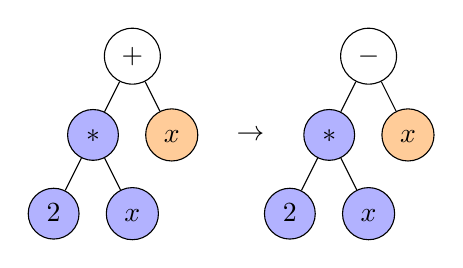
\begin{tikzpicture}
    \node[varnode] (del_plus) {$+$};
    \node[varnode, colorA] (del_times) at ($(del_plus)+(-0.5,-1)$) {$*$};
    \node[varnode, colorB] (del_one) at ($(del_plus)+(0.5,-1)$) {$x$};
    \node[varnode, colorA] (del_two) at ($(del_times)+(-0.5,-1)$) {$2$};
    \node[varnode, colorA] (del_three) at ($(del_times)+(0.5,-1)$) {$x$};
    \draw (del_plus) -- (del_times);
    \draw (del_plus) -- (del_one);
    \draw (del_times) -- (del_two);
    \draw (del_times) -- (del_three);

    \node[varnode] (ins_minus) at ($(del_plus)+(3,0)$) {$-$};
    \node[varnode, colorA] (ins_times) at ($(ins_minus)+(-0.5,-1)$) {$*$};
    \node[varnode, colorB] (ins_one) at ($(ins_minus)+(0.5,-1)$) {$x$};
    \node[varnode, colorA] (ins_two) at ($(ins_times)+(-0.5,-1)$) {$2$};
    \node[varnode, colorA] (ins_three) at ($(ins_times)+(0.5,-1)$) {$x$};
    \draw (ins_minus) -- (ins_times);
    \draw (ins_minus) -- (ins_one);
    \draw (ins_times) -- (ins_two);
    \draw (ins_times) -- (ins_three);

    \node (arrow) at ($(del_one)!0.5!(ins_times)$) {$\rightarrow$};
\end{tikzpicture}
\end{minipage}\hfill
\begin{minipage}{0.49\textwidth}
\centering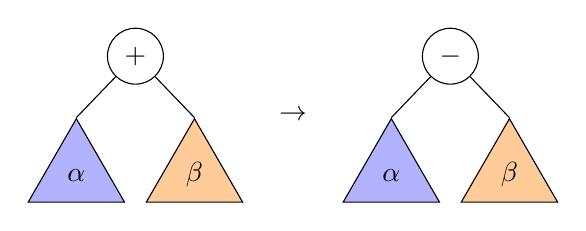
\begin{tikzpicture}
    \node[varnode] (del_plus) {$+$};
    \node[mvnode, colorA] (del_alpha) at ($(del_plus)+(-0.75,-1.5)$) {$\alpha$};
    \node[mvnode, colorB] (del_beta) at ($(del_plus)+(0.75,-1.5)$) {$\beta$};
    \draw (del_plus) -- (del_alpha.north);
    \draw (del_plus) -- (del_beta.north);

    \node[varnode] (ins_minus) at ($(del_plus)+(4,0)$) {$-$};
    \node[mvnode, colorA] (ins_alpha) at ($(ins_minus)+(-0.75,-1.5)$) {$\alpha$};
    \node[mvnode, colorB] (ins_beta) at ($(ins_minus)+(0.75,-1.5)$) {$\beta$};
    \draw (ins_minus) -- (ins_alpha.north);
    \draw (ins_minus) -- (ins_beta.north);

    \node (arrow) at ($($(del_beta)!0.5!(del_plus)$)!0.5!($(ins_alpha)!0.5!(ins_minus)$)$) {$\rightarrow$};
\end{tikzpicture}
\end{minipage}
\label{fig:metavar_elision}
\caption{The change \st{$(2*x)+x$} $\rightarrow$ \ul{$(2*x)-x$} becomes \st{$\alpha+\beta$} $\rightarrow$ \ul{$\alpha-\beta$} after meta-variable elision.}
\end{figure}

Trying to merge together two nodes in the AST is easy, we simply need to check if they use the same root constructor, recursively merge if it is the case, and fail otherwise. However, this approach is really bad with sequences (eg. sequences of functions or sequences of statements). We do not want to fully split a list if only one element has been inserted, removed or changed. Therefore, we use list edit scripts instead as the output of a merge operation on two sequences. We call the merged part of the difference tree its spine.

\begin{figure}[ht]
\begin{minipage}{0.49\textwidth}
\centering\begin{tikzpicture}
    \node[varnode, deleted] (del_block) {$\{\ldots\}$};
    \node[varnode, deleted] (del_stmt1) at ($(del_block)+(-1,-1)$) {$\textbf{let}$};
    \node[varnode, deleted] (del_stmt2) at ($(del_block)+(1,-1)$) {$=$};
    \node[varnode, deleted] (del_x) at ($(del_stmt1)+(-0.5,-1)$) {$x$};
    \node[varnode, deleted] (del_three) at ($(del_stmt1)+(0.5,-1)$) {$3$};
    \node[varnode, deleted] (del_y) at ($(del_stmt2)+(-0.5,-1)$) {$y$};
    \node[varnode, deleted] (del_yx) at ($(del_stmt2)+(0.5,-1)$) {$x$};
    \draw (del_block) -- (del_stmt1);
    \draw (del_block) -- (del_stmt2);
    \draw (del_stmt1) -- (del_x);
    \draw (del_stmt1) -- (del_three);
    \draw (del_stmt2) -- (del_y);
    \draw (del_stmt2) -- (del_yx);

    \node[varnode, inserted] (ins_block) at ($(del_plus)+(4.25,0)$) {$\{\ldots\}$};
    \node[varnode, inserted] (ins_stmt1) at ($(ins_block)+(-1,-1)$) {$=$};
    \node[varnode, inserted] (ins_stmt2) at ($(ins_block)+(1,-1)$) {$=$};
    \node[varnode, inserted] (ins_y) at ($(ins_stmt1)+(-0.5,-1)$) {$y$};
    \node[varnode, inserted] (ins_five) at ($(ins_stmt1)+(0.5,-1)$) {$5$};
    \node[varnode, inserted] (ins_z) at ($(ins_stmt2)+(-0.5,-1)$) {$z$};
    \node[varnode, inserted] (ins_nine) at ($(ins_stmt2)+(0.5,-1)$) {$9$};
    \draw (ins_block) -- (ins_stmt1);
    \draw (ins_block) -- (ins_stmt2);
    \draw (ins_stmt1) -- (ins_y);
    \draw (ins_stmt1) -- (ins_five);
    \draw (ins_stmt2) -- (ins_z);
    \draw (ins_stmt2) -- (ins_nine);

    \node (arrow) at ($(del_stmt2)!0.5!(ins_stmt1)$) {$\rightarrow$};
\end{tikzpicture}
\end{minipage}\hfill
\begin{minipage}{0.45\textwidth}
\centering\begin{tikzpicture}
    \node[varnode] (spine_block) {$\{\ldots\}$};
    \node[modnode, scale=0.8, deleted] (spine_stmt1) at ($(spine_block)+(-2.5,-1.5)$) {\tikz{
        \node[varnode] (del_stmt) {$\textbf{let}$};
        \node[varnode] (del_x) at ($(del_stmt)+(-0.5,-1)$) {$x$};
        \node[varnode] (del_three) at ($(del_stmt)+(0.5,-1)$) {$3$};
        \draw (del_stmt) -- (del_x);
        \draw (del_stmt) -- (del_three);
    }};
    \node[varnode] (spine_stmt2) at ($(spine_block)+(-0.25,-1)$) {$=$};
    \node[modnode, scale=0.8, inserted] (spine_stmt3) at ($(spine_block)+(2.5,-1.5)$) {\tikz{
        \node[varnode] (ins_stmt) at ($(ins_block)+(1,-1)$) {$=$};
        \node[varnode] (ins_z) at ($(ins_stmt)+(-0.5,-1)$) {$z$};
        \node[varnode] (ins_nine) at ($(ins_stmt)+(0.5,-1)$) {$9$};
        \draw (ins_stmt) -- (ins_z);
        \draw (ins_stmt) -- (ins_nine);
    }};{};
    \node[varnode] (spine_y) at ($(spine_stmt2)+(-0.75,-1)$) {$y$};
    \node[modnode, scale=0.8] (change_y) at ($(spine_stmt2)+(0.75,-1)$) {\tikz{
        \node[varnode, deleted] (x) {$x$};
        \node[varnode, inserted] (five) at ($(x)+(1.2,0)$) {$5$};
        \node (arrow) at ($(x)!0.5!(five)$) {$\rightarrow$};
    }};
    \draw (spine_block) -- (spine_stmt1);
    \draw (spine_block) -- (spine_stmt2);
    \draw (spine_block) -- (spine_stmt3);
    \draw (spine_stmt2) -- (spine_y);
    \draw (spine_stmt2) -- (change_y);
\end{tikzpicture}
\end{minipage}
\label{fig:spine_seq_align}
\caption{The change \st{$\{ \mathbf{let}\ x=3; y=5\}$} $\rightarrow$ \ul{$\{ y=5; z=9 \}$} becomes $\{\text{\st{$\mathbf{let}\ x=3;$}}\ y = \text{\st{$x$}} \rightarrow \text{\ul{$5$}}; \text{\ul{$z = 9$}}\}$ after spine merging and sequence alignment.}
\end{figure}

We denote by $S(\overrightarrow{t}, \overrightarrow{s})$ a constructor from the target language AST, with an arbitrary but fixed arity of trees ($t$) and sequences ($s$). For instance one of the possible $S$ could be the language construction \lstinline[mathescape]|if $t_{cond}$ { $\overrightarrow{s_{true}}$ } else { $\overrightarrow{s_{false}}$ }| with one expression sub-tree and two nested sequences of instructions.

This gives the following types for difference trees:
\begin{align*}
c &::= S(\overrightarrow{c}, \overrightarrow{c}) \typsep \alpha\\
t &::= S(\overrightarrow{t}, \overrightarrow{s}) \typsep \square \typsep \text{\st{$c$}} \rightarrow \text{\ul{$c$}}\\
s &::= t \typsep \text{\st{$c$}} \typsep \text{\ul{$c$}}\\
\end{align*}

Here $\square$ represent a hole for unchanged sub-tree, \st{strike through} represent deleted code, and \ul{underlines} represent insertions.

\subsubsection{Computing a syntactic difference}
To compute a syntactic difference, we take ASTs of both the original and the modified program and we run the following algorithm:
\begin{itemize}
  \item Compute a hash for each node of each AST.
  \item Take the subset of hashes occurring both in original and modified AST.
  \item Elide the nodes with a hash in the subset to remember just their hash.
  \item If an elided node does not match an elision with the same hash in the other tree, replace it by the original sub-tree.
  \item Merge both AST into a common spine where possible, else keep changes as two separate elided trees. Always try to align sequences using recursively a dynamic algorithm minimizing the number of nodes of the resulting tree.
  \item Replace each hash by a meta-variable letter (just an index in code), and replace changes $\text{\st{$\alpha$}} \rightarrow \text{\ul{$\alpha$}}$ by $\square$ when $\alpha$ does not occur elsewhere.
\end{itemize}

This algorithm is in $O(nm)$ where $n$ (resp. $m$) is the number of node of the original (resp. modified) tree. The most computationally expansive part of the algorithm is computing sequence alignments, all the rest is linear.

\subsubsection{Applying syntactic differences}
We can see syntactic differences as partial functions turning a syntax tree into another syntax tree.
The difference between $d$ and $i$ is therefore a function that is at least mapping $d$ into $i$, but it is also defined on some other trees sharing all the relevant structure with $d$.

The implied function of a difference tree is defined as follows: let's suppose that we have $\Gamma$ a function from meta-variable inside the difference tree, to syntax trees, given by an oracle. In practice, $\Gamma$ is constrained enough to be inferred. Then apply the following syntax driven rules:

\noindent
\begin{minipage}{.49\textwidth}
\begin{prooftree}
 \AxiomC{}
 \RightLabel{\textsc{Id}}
 \UnaryInfC{$\Gamma \vdash \square(t) = t$}
\end{prooftree}

\begin{prooftree}
 \AxiomC{$\Gamma \vdash d(t)$}
 \RightLabel{\textsc{Change}}
 \UnaryInfC{$\Gamma \vdash (\text{\st{$d$}} \rightarrow \text{\ul{$i$}})(t) = \Gamma(i)$}
\end{prooftree}

\begin{prooftree}
 \AxiomC{$\overrightarrow{\Gamma \vdash t(d_t) = i_t}$}
 \AxiomC{$\overrightarrow{\Gamma \vdash s(d_s) = i_s}$}
 \RightLabel{\textsc{Spine}}
 \BinaryInfC{$\Gamma \vdash S(\overrightarrow{t},\overrightarrow{s})(S(\overrightarrow{d_t},\overrightarrow{d_s})) = S(\overrightarrow{i_t}, \overrightarrow{i_s})$}
\end{prooftree}

\begin{prooftree}
 \AxiomC{$\Gamma \vdash t(d) = i$}
 \AxiomC{$\Gamma \vdash r(d_r) = i_r$}
 \RightLabel{\textsc{SeqZip}}
 \BinaryInfC{$\Gamma \vdash (t::r)(d::d_r) = i::i_r$}
\end{prooftree}
\end{minipage}
\begin{minipage}{.49\textwidth}
\begin{prooftree}
 \AxiomC{$\Gamma \vdash c(d)$}
 \AxiomC{$\Gamma \vdash r(d_r) = i_r$}
 \RightLabel{\textsc{SeqDel}}
 \BinaryInfC{$\Gamma \vdash (\text{\st{$c$}}::r)(d::d_r) = i_r$}
\end{prooftree}

\begin{prooftree}
 \AxiomC{$\Gamma \vdash r(d_r) = i_r$}
 \RightLabel{\textsc{SeqIns}}
 \UnaryInfC{$\Gamma \vdash (\text{\ul{$c$}}::r)(d_r) = \Gamma(c) :: i_r$}
\end{prooftree}

\begin{prooftree}
 \AxiomC{$\Gamma(\alpha) = d$}
 \RightLabel{\textsc{DelMv}}
 \UnaryInfC{$\Gamma \vdash \alpha(d)$}
\end{prooftree}

\begin{prooftree}
 \AxiomC{$\overrightarrow{\Gamma \vdash c_t(d_t)}$}
 \AxiomC{$\overrightarrow{\Gamma \vdash c_s(d_s)}$}
 \RightLabel{\textsc{DelSyn}}
 \BinaryInfC{$\Gamma \vdash S(\overrightarrow{c_t}, \overrightarrow{c_s})(S(\overrightarrow{d_t}, \overrightarrow{d_s}))$}
\end{prooftree}
\end{minipage}

\subsubsection{Practical considerations: how to extend a syntax tree}
Implementing an algorithm that requires extending a syntax tree can be tidious in practice because we want to attach new information and/or create holes on a fixed structure while keeping the typedness of the tree.

Along this paper, I give a Rust implementation for the syntax difference and merging algorithm of Rust codes. The parser used (the syn crate) uses more than 180 types in its syntax trees, so manual extension was not an option.

The solution I give is based on a somehow generic code generation system (implemented as procedural macro). The idea is that we want to add the ability to extend a type family of mutually recursive sum of products (nested enums and structs in Rust terminology) by changing systematically some types by others inside it, thus generating a new family variant. Then, we also make a code generator to browse through or convert between variants of the same family. After generation, manual code is only required for the new structures of the trees.

\begin{lstlisting}[label=lst:codegen, caption={Usage example of the code generator for creating the hash-tagged family variant}]
syn_codegen! {
    pub mod hash {
        use crate::family_traits::Convert;
        use crate::hash_tree::{HashTagged, TreeHasher};

        #[derive(Hash, Eq, PartialEq)]
        extend_family! {
            Expr as HashTagged<Expr>,
            Vec<Stmt> as Vec<HashTagged<Stmt>>,
            Vec<Item> as Vec<HashTagged<Item>>,
            [...] // other type replacements
        }

        family_impl!(Convert<syn, self> for TreeHasher);
    }

    [...] // other family variants
}
\end{lstlisting}


Note that for having a production ready tool, the current parser is not adapted, as it systematically forgets the comments inside source code. But this is left for future work as a pure engeneering problem.

\subsection{Awareness colors}

Before merging differences together, we want to define a way of keeping track of which commit introduced each modification. For that we use a notion of awareness colors.

Each commit in a fusion get an associated tint. If we denote by $\mathbb{T}$ the set of all tints considered, we can define the color set as $\mathbb{C} = \mathcal{P}(\mathbb{T})$. This forms the complete lattice $(\mathbb{C}, \cup, \cap, \subset)$. We name the maximum in this lattice white (equal to $\mathbb{T}$, denoted $\top$) and the minimum black (equal to $\emptyset$, denoted $\bot$).

A modification gets the color $c \in \mathbb{C}$, if for all tint in $c$, the associated commit is aware of the presence of the colored source code.

The white color having all the tints, it represent a consensus of all the commits. On the other side, black represent the fact that no single commit can claim responsibility for a given value. This makes the white color the good choice for everything already present in the original file, and black a color that we want to track and avoid.

Both code and modification can carry colors. Code has the color of the commits that introduced it, or is white if it comes from the original file. The same code can be introduced twice if the exact same insertion has been done by multiple commits. In this case it will have the union of both tints as its color. Similarly, insertions and deletions have the color of all the commits that made them.

Before merging, we apply the singleton color corresponding to the commit on the difference tree recursively as follows:
\begin{align*}
{\color{red}c} &= {\color{red}S(\overrightarrow{c}, \overrightarrow{c})} \typsep \alpha\\
{\color{red}t} &= S(\overrightarrow{\color{red}t}, \overrightarrow{\color{red}s}) \typsep \square \typsep \text{\setstcolor{red}\st{$c$}} \rightarrow \text{\color{red}\ul{$c$}}\\
{\color{red}s} &= {\color{red}t} \typsep \text{\setstcolor{red}\st{$c$}} \typsep \text{\color{red}\ul{$c$}}\\
\end{align*}

Note that meta-variables and holes are never colored, and that AST structures are not colored in the spine but are in the inserted sub-trees. This reflects the fact that in the spine and inside holes, code comes from the original source code, while elsewhere it is introduced by the commit.

\subsection{Merging differences}
Now that we have difference trees for each individual concurrent change, we can try to merge them in a way that keeps track of the origin of each piece of code.

However, as with line based merge, this merging operation can and will regularly fail if someone wants to merge syntactically incompatible changes.

We therefore break the symmetry between deletion and insertion trees as there will be only one deletion and multiple insertions, and we need to extend our difference types to accumulate potential conflicts.

\begin{align*}
d &::= S(\overrightarrow{d}, \overrightarrow{d}) \typsep \alpha \typsep MvConflict(\alpha, d, i) \\
i &::= S(\overrightarrow{i}, \overrightarrow{j}) \typsep \alpha \typsep Conflict(\overrightarrow{i})\\
j &::= i \typsep DelConflict(i) \typsep OrdConflict(\overrightarrow{i})\\
t &::= S(\overrightarrow{t}, \overrightarrow{s}) \typsep \square \typsep  \text{\st{$d$}} \rightarrow \text{\ul{$i$}}\\
s &::= t \typsep \text{\st{$d$}} \typsep DelConflict(d, i) \typsep \text{\ul{$i$}} \typsep OrdConflict(\overrightarrow{\overrightarrow{i}})\\
\end{align*}

When dealing with meta-variables, that represent a multi-source multi-target code move, our merging algorithm will try to push changes toward the destination of the code movement.
This is done in a two-phase way. First, if we have two changes facing each other we try to inline one of them inside the deletion tree of the other, by allowing differences wherever we have a meta-variable. To avoid making any arbitrary choice, this is ignored if both changes could be inlined in the other. Then, we check that these inlined changes are consistent for each meta-variable, and if they are, we replace all occurrences of the meta-variable by the obtained insertion.

In absence of conflicts, merged differences have the same semantics as simple difference trees.

Conflict represent parts that couldn't be merged and therefore prevent application of the difference on any tree. They can come from four different sources:
\begin{itemize}
  \item $Conflict$ simply represent two different insertions that were in the same place.
  \item $DelConflict$ appears where one commit deletes a node while the other one had changes in it.
  \item $OrdConflict$ is caused by two insertions taking place at the same location. As the merge operation is never performing any choice, it cannot arbitrarily order them.
  \item $MvConflict$ is triggered when a meta-variable appears more than once in deletion tree, and the inlined insertions in each occurrences differ, therefore not giving a consistent replacement.
\end{itemize}

The application domain of the merged difference $t_1 \circ t_2$ is the intersection of the domains of $t_1$ and $t_2$ in absence of conflicts.
Also we ensure that $t \circ t = t$.

\subsubsection{Specification of the difference merging algorithm}
The difference merging algorithm is defined modulo two replacement functions $\Gamma$ and $\Delta$ from meta-variable to respectively insertion and deletion trees, that are heavily constrained and in practice inferred during the merge.

\begin{prooftree}
 \AxiomC{$\Gamma, \Delta \vdash t_r \circ t_l = t$}
 \UnaryInfC{$\Gamma, \Delta \vdash t_l \circ t_r = t$}
\end{prooftree}

\paragraph{Merge spine nodes}
\begin{prooftree}
 \AxiomC{}
 \UnaryInfC{$\Gamma, \Delta \vdash t \circ id = \Delta(\Gamma(t))$}
\end{prooftree}

\begin{prooftree}
 \AxiomC{$\overrightarrow{\Gamma, \Delta \vdash t_l \circ t_r = t}$}
 \UnaryInfC{$\Gamma, \Delta \vdash S(\overrightarrow{t_l}) \circ S(\overrightarrow{t_r}) = S(\overrightarrow{t})$}
\end{prooftree}

\begin{prooftree}
 \AxiomC{$\Gamma \vdash i_l \not\subset d_r$}
 \AxiomC{$\Gamma \vdash i_r \not\subset d_l$}
 \AxiomC{$\Gamma \vdash d_l$}
 \AxiomC{$\Gamma \vdash d_r$}
 \QuaternaryInfC{$\Gamma, \Delta \vdash (d_l, i_l) \circ (d_r, i_r) = (d_l \wedge d_r, i_l \vee i_r)$}
\end{prooftree}

\begin{prooftree}
 \AxiomC{$\Gamma \vdash i_l \subset d_r = d'$}
 \AxiomC{$\Gamma \vdash i_r \not\subset d_l$}
 \AxiomC{$\Gamma \vdash d_l$}
 \TrinaryInfC{$\Gamma, \Delta \vdash (d_l, i_l) \circ (d_r, i_r) = (d' \wedge d_l, \Gamma(i_r))$}
\end{prooftree}

\begin{prooftree}
 \AxiomC{$\Gamma \vdash i_l \subset d_r$}
 \AxiomC{$\Gamma \vdash i_r \subset d_l$}
 \AxiomC{$\Gamma \vdash d_l$}
 \AxiomC{$\Gamma \vdash d_r$}
 \QuaternaryInfC{$\Gamma, \Delta \vdash (d_l, i_l) \circ (d_r, i_r) = (d_l \wedge d_r, i_l \vee i_r)$}
\end{prooftree}

\paragraph{Merge sequence edit scripts (except insertions)}
\begin{prooftree}
 \AxiomC{$\Gamma, \Delta \vdash t_l \circ t_r = t$}
 \AxiomC{$\Gamma, \Delta \vdash r_l \circ r_r = r$}
 \BinaryInfC{$\Gamma, \Delta \vdash (Zip(t_l) :: r_l) \circ (Zip(t_r) :: r_r) = Zip(t) :: r$}
\end{prooftree}

\begin{prooftree}
 \AxiomC{$\Gamma \vdash d_l$}
 \AxiomC{$\Gamma \vdash d_r$}
 \AxiomC{$\Gamma, \Delta \vdash r_l \circ r_r = r$}
 \TrinaryInfC{$\Gamma, \Delta \vdash (Del(d_l) :: r_l) \circ (Del(d_r) :: r_r) = Del(d_l \wedge d_r) :: r$}
\end{prooftree}

\begin{prooftree}
 \AxiomC{$t_r = (d_r, i_r)$}
 \AxiomC{$\Gamma \vdash i_r \subset d_l$}
 \AxiomC{$\Gamma \vdash d_r$}
 \AxiomC{$\Gamma, \Delta \vdash r_l \circ r_r = r$}
 \QuaternaryInfC{$\Gamma, \Delta \vdash (Del(d_l) :: r_l) \circ (Zip(t_r) :: r_r) = Del(d_l \wedge d_r) :: r$}
\end{prooftree}

\begin{prooftree}
 \AxiomC{$t_r = (d_r, i_r)$}
 \AxiomC{$\Gamma \vdash i_r \not\subset d_l$}
 \AxiomC{$\Gamma \vdash d_l$}
 \AxiomC{$\Gamma \vdash d_r$}
 \AxiomC{$\Gamma, \Delta \vdash r_l \circ r_r = r$}
 \QuinaryInfC{$\Gamma, \Delta \vdash (Del(d_l) :: r_l) \circ (Zip(t_r) :: r_r) = DelConflict(d_l \wedge d_r, \Gamma(i_r)) :: r$}
\end{prooftree}

\begin{prooftree}
 \AxiomC{$\Gamma \vdash i_l \not\subset d_r$}
 \AxiomC{$\Gamma \vdash i_r \not\subset d_l$}
 \AxiomC{$\Gamma \vdash d_l$}
 \AxiomC{$\Gamma \vdash d_r$}
 \AxiomC{$\Gamma, \Delta \vdash r_l \circ r_r = r$}
 \QuinaryInfC{$\Gamma, \Delta \vdash (DelConflict(d_l, i_l) :: r_l) \circ (DelConflict(d_r, i_r) :: r_r) = DelConflict(d_l \wedge d_r, i_l \vee i_r) :: r$}
\end{prooftree}

\begin{prooftree}
 \AxiomC{$\Gamma \vdash i_l \subset d_r = d'_r$}
 \AxiomC{$\Gamma \vdash i_r \not\subset d_l$}
 \AxiomC{$\Gamma \vdash d_l$}
 \AxiomC{$\Gamma, \Delta \vdash r_l \circ r_r = r$}
 \QuaternaryInfC{$\Gamma, \Delta \vdash (DelConflict(d_l, i_l) :: r_l) \circ (DelConflict(d_r, i_r) :: r_r) = DelConflict(d_l \wedge d'_r, \Gamma(i_r)) :: r$}
\end{prooftree}

\begin{prooftree}
 \AxiomC{$\Gamma \vdash i_l \subset d_r = d'_r$}
 \AxiomC{$\Gamma \vdash i_r \subset d_l = d'_l$}
 \AxiomC{$\Gamma, \Delta \vdash r_l \circ r_r = r$}
 \TrinaryInfC{$\Gamma, \Delta \vdash (DelConflict(d_l, i_l) :: r_l) \circ (DelConflict(d_r, i_r) :: r_r) = Del(d'_l \wedge d'_r) :: r$}
\end{prooftree}

\begin{prooftree}
 \AxiomC{$t_r = (d_r, i_r)$}
 \AxiomC{$\Gamma, \Delta \vdash (DelConflict(d_l, i_l) :: r_l) \circ (DelConflict(d_r, i_r) :: r_r) = r$}
 \BinaryInfC{$\Gamma, \Delta \vdash (DelConflict(d_l, i_l) :: r_l) \circ (Zip(t_r) :: r_r) = r$}
\end{prooftree}

\begin{prooftree}
 \AxiomC{$\Gamma \vdash i_l \not\subset d_r$}
 \AxiomC{$\Gamma \vdash d_r$}
 \AxiomC{$\Gamma \vdash d_l$}
 \AxiomC{$\Gamma, \Delta \vdash r_l \circ r_r = r$}
 \QuaternaryInfC{$\Gamma, \Delta \vdash (DelConflict(d_l, i_l) :: r_l) \circ (Del(d_r) :: r_r) = DelConflict(d_l \wedge d_r, \Gamma(i_l)) :: r$}
\end{prooftree}

\begin{prooftree}
 \AxiomC{$\Gamma \vdash i_l \subset d_r = d'_r$}
 \AxiomC{$\Gamma \vdash d_l$}
 \AxiomC{$\Gamma, \Delta \vdash r_l \circ r_r = r$}
 \TrinaryInfC{$\Gamma, \Delta \vdash (DelConflict(d_l, i_l) :: r_l) \circ (Del(d_r) :: r_r) = Del(d_l \wedge d'_r) :: r$}
\end{prooftree}

\paragraph{Merge insertions in sequence edit scripts}

\begin{prooftree}
 \AxiomC{$s_r \neq Ins(\_)$}
 \AxiomC{$s_r \neq OrdConflict(\_)$}
 \AxiomC{$\Gamma, \Delta \vdash r_l \circ (s_r :: r_r) = r$}
 \TrinaryInfC{$\Gamma, \Delta \vdash (Ins(i_l) :: r_l) \circ (s_r :: r_r) = Ins(\Gamma(i_l)) :: r$}
\end{prooftree}

\begin{prooftree}
 \AxiomC{$\Gamma(i_l) = \Gamma(i_r) = i$}
 \AxiomC{$\Gamma, \Delta \vdash r_l \circ r_r = r$}
 \BinaryInfC{$\Gamma, \Delta \vdash (Ins(i_l) :: r_l) \circ (Ins(i_r) :: r_r) = Ins(i) :: r$}
\end{prooftree}

\begin{prooftree}
 \AxiomC{$\Gamma, \Delta \vdash r_l \circ r_r = r$}
 \UnaryInfC{$\Gamma, \Delta \vdash (Ins(i_l) :: r_l) \circ (Ins(i_r) :: r_r) = OrdConflict([\Gamma(i_l), \Gamma(i_r)]) :: r$}
\end{prooftree}

\begin{prooftree}
 \AxiomC{$s_r \neq Ins(\_)$}
 \AxiomC{$s_r \neq OrdConflict(\_)$}
 \AxiomC{$\Gamma, \Delta \vdash r_l \circ (s_r :: r_r) = r$}
 \TrinaryInfC{$\Gamma, \Delta \vdash (OrdConflict(i_l) :: r_l) \circ (s_r :: r_r) = OrdConflict(\Gamma(i_l)) :: r$}
\end{prooftree}

\begin{prooftree}
 \AxiomC{$\Gamma, \Delta \vdash r_l \circ r_r = r$}
 \UnaryInfC{$\Gamma, \Delta \vdash (Ins(i_l) :: r_l) \circ (OrdConflict(i_r) :: r_r) = OrdConflict(\Gamma(i_l) :: \Gamma(i_r)) :: r$}
\end{prooftree}

\begin{prooftree}
 \AxiomC{$\Gamma, \Delta \vdash r_l \circ r_r = r$}
 \UnaryInfC{$\Gamma, \Delta \vdash (OrdConflict(i_l) :: r_l) \circ (OrdConflict(i_r) :: r_r) = OrdConflict(\Gamma(i_l) @ \Gamma(i_r)) :: r$}
\end{prooftree}

\paragraph{Inclusion of insertion inside a deletion}

\begin{prooftree}
 \AxiomC{$\overrightarrow{\Gamma \vdash i \subset d = d'}$}
 \UnaryInfC{$\Gamma \vdash S(\overrightarrow{i}) \subset S(\overrightarrow{d}) = S(\overrightarrow{d'})$}
\end{prooftree}

\begin{prooftree}
 \AxiomC{$\Gamma(\alpha) = \Gamma(i)$}
 \UnaryInfC{$\Gamma \vdash i \subset \alpha = \alpha$}
\end{prooftree}

\begin{prooftree}
 \AxiomC{$\Gamma(\alpha) = \top$}
 \UnaryInfC{$\Gamma \vdash i \subset \alpha = MvConflict(\alpha, \alpha, i)$}
\end{prooftree}

\begin{prooftree}
 \AxiomC{$\Gamma(\alpha) = \top$}
 \UnaryInfC{$\Gamma \vdash i \subset MvConflict(\alpha, d, i') = MvConflict(\alpha, d, i \vee i')$}
\end{prooftree}

\begin{prooftree}
 \AxiomC{$d \neq \alpha$}
 \AxiomC{$d \neq S(\_)$}
 \BinaryInfC{$\Gamma \vdash S(\_) \not\subset d$}
\end{prooftree}

\begin{prooftree}
 \AxiomC{$d \neq \alpha$}
 \AxiomC{$i \neq S(\_)$}
 \BinaryInfC{$\Gamma \vdash i \not\subset d$}
\end{prooftree}

\paragraph{Coherence with $\Gamma$ of kept deletion trees}

\begin{prooftree}
 \AxiomC{$\overrightarrow{\Gamma \vdash d}$}
 \UnaryInfC{$\Gamma \vdash S(\overrightarrow{d})$}
\end{prooftree}

\begin{prooftree}
 \AxiomC{$\Gamma(\alpha) \in \{ \oplus(\Delta(\alpha)), \top \}$}
 \UnaryInfC{$\Gamma \vdash \alpha$}
\end{prooftree}

Where $\oplus$ is a function transposing a deletion tree to an insertion tree by passing through each $MvConflict$ constructor so that $\oplus(MvConflict(\alpha, d, i)) = \oplus(d)$.

\begin{prooftree}
 \AxiomC{$\Gamma(\alpha) = \top$}
 \AxiomC{$\Gamma \vdash d$}
 \BinaryInfC{$\Gamma \vdash MvConflict(\alpha, d, i)$}
\end{prooftree}

\paragraph{Deletion intersection}
\begin{prooftree}
 \AxiomC{$\overrightarrow{\Delta \vdash d_l \wedge d_r = d}$}
 \UnaryInfC{$\Delta \vdash S(\overrightarrow{d_l}) \wedge S(\overrightarrow{d_r}) = S(\overrightarrow{d})$}
\end{prooftree}

\begin{prooftree}
 \AxiomC{}
 \UnaryInfC{$\Delta \vdash \alpha \wedge \alpha = \Delta(\alpha)$}
\end{prooftree}

\begin{prooftree}
 \AxiomC{$\Delta \vdash \Delta(\alpha) \wedge d_r = \Delta(\alpha)$}
 \UnaryInfC{$\Delta \vdash \alpha \wedge d_r = \Delta(\alpha)$}
\end{prooftree}

\begin{prooftree}
 \AxiomC{$\Delta \vdash \Delta(\alpha) \wedge d_l = \Delta(\alpha)$}
 \UnaryInfC{$\Delta \vdash d_l \wedge \alpha = \Delta(\alpha)$}
\end{prooftree}

\begin{prooftree}
 \AxiomC{$\Delta \vdash d_l \wedge d_r = d$}
 \UnaryInfC{$\Delta \vdash d_l \wedge MvConflict(\alpha, d_r, i) = MvConflict(\alpha, d, \Gamma(i))$}
\end{prooftree}

\begin{prooftree}
 \AxiomC{$\Delta \vdash d_l \wedge d_r = d$}
 \UnaryInfC{$\Delta \vdash MvConflict(\alpha, d_l, i) \wedge d_r = MvConflict(\alpha, d, \Gamma(i))$}
\end{prooftree}

\paragraph{Simplification of insertion union}

\begin{prooftree}
 \AxiomC{$\Gamma(i_l) = \Gamma(i_r) = i$}
 \UnaryInfC{$\Gamma \vdash i_l \vee i_r = i$}
\end{prooftree}

\begin{prooftree}
 \AxiomC{$\overrightarrow{\Gamma \vdash i_l \vee i_r = i}$}
 \UnaryInfC{$\Gamma \vdash S(\overrightarrow{i_l}) \vee S(\overrightarrow{i_r}) = S(\overrightarrow{i})$}
\end{prooftree}

\begin{prooftree}
 \AxiomC{}
 \UnaryInfC{$\Gamma \vdash i_l \vee i_r = Conflict(\Gamma(i_l), \Gamma(i_r))$}
\end{prooftree}

\subsection{Algorithm for merging differences}
The above specification is telling what a merged version must look like but doesn't tell how to compute this merged version. Simply following the rules is not enough, because we have two global variables $\Gamma$ and $\Delta$ to infer. Moreover, for $\Gamma$ there is a priori several possibilities. Hopefully, we can easily distinguish one that will minimize the number of conflicts generated. We want a valid $\Gamma$ that minimize the number of meta-variables associated to $\top$.

From a high level point of view, the merging algorithm follows these steps:
\begin{itemize}
 \item Ensure that all the meta-variables used in both programs are disjoint by alpha-renaming whenever necessary.
 \item Align the spines of both difference trees. This requires unrolling whenever one of the difference tree still has a spine node while the other has a difference at the same place. This step also aligns the sequences and detect insert order conflicts. \todo{Figure here?}
 \item Merge the insertion trees together. For each insertion we try to inline it inside the facing deletion tree first. If only one inlining could succeed, then we perform it, else we try to merge together the insertion trees. This take the union of tints as resulting color and create conflicts whenever both insertion do not match. By performing inlinings, we can remember $\Gamma^*$ a map form meta-variables to a list of the trees that were inlined on the metavariable.
 \item Merge the deletion trees together. For that, we build $\Delta$ as we merge the sub-trees.
 \item Then we perform all the substitutions wherever there are meta-variables with a replacement in $\Delta$ for deletion trees, and in $\Gamma$ for insertion trees.
\end{itemize}

If we want to merge more than two differences, we can reapply the same algorithm on already merged trees, thus accumulating modifications but also conflicts.

\section{Semantic merge}
Having two commits syntactically merged do not mean that the result is a valid semantic combination that respect the intentions of all original committers.

\todo{Example du double +1 syntaxiquement valide mais sémantiquement incorrect}

That's why after the syntax merging step, we also want to check the semantic of the fusion.

In this section we will show that first non-conflicting difference trees can be interpreted as correlation oracles between the original code and a merged candidate. And secondly that we can derive a runtime analysis that ensures that there is no unresolved ambiguity introduced by the fusion operation. In future works, this runtime analysis could be refined into a static analysis.

If we combine this invariant with the fact that the fusion never lose any introduced change, we obtain the certainty that the intentions inside all original commits are respected, because both changes and implicit environment assumptions are preserved.

\subsection{Interpreting a difference tree as a correlation oracle}
\subsubsection{Definition of a correlation oracle}
\todo{Write this or maybe just quote T. Girka thesis}

\subsubsection{Operational semantics of the studied language}
In this paper, we will use the following programming language, a simplified version of Rust. It has been chosen because it allows us to explore both functional and imperative coding styles, and we stripped all the borrowing and trait systems that could be difficult to understand for a reader without any Rust background.

\newcommand{\ident}{\mathbb{I}}
\newcommand{\typ}{\mathbb{T}}
Syntactically, with $\ident$ the set of variable and function identifiers, $\typ$ the set of type identifiers and $\diamond$ (resp. $\star$) the set of primitive binary (resp. unary) functions, it is defined by:
\begin{align*}
program &::= \boxed{item}^*\\
item &::= func \typsep enum\\
enum &::= \mathbf{enum}\ \typ\ \{ \boxed{\ident(\boxed{\typ,}^*),}^* \}\\
func &::= \mathbf{fn}\ \ident(\boxed{\ident: \typ}^*) \rightarrow \typ\ block\\
block &::= \{ \boxed{expr;}^* expr \}\\
expr &::= \ident \typsep literal \typsep \star expr \typsep expr \diamond expr \typsep \ident = expr \typsep \ident(\boxed{expr}^*) \typsep block \typsep \mathbf{if}\ expr\ block\ \mathbf{else}\ block\\
&\typsep \mathbf{while}\ expr\ block \typsep \mathbf{match}\ expr\ \{ \boxed{\ident(\boxed{\ident,}^*) \Rightarrow expr,}^* \} \typsep \mathbf{continue} \typsep \mathbf{break} \typsep \textbf{return}\ expr\\
literal &::= () \typsep \mathbf{true} \typsep \mathbf {false} \typsep \mathbb{Z}
\end{align*}

To define the semantics, we give the program state as a tuple $\langle\kappa, v, S\rangle$ where $\kappa$ is the continuation, $v$ the value of the last computed expression and $S$ the local store stack. For function calls, we can push a new store on the previous one, only the topmost store can be used and updated as it correspond to the current function.

We also keep the set of constructors, and the set of function as a global state. We denote $\mathbb{G}(f)$ the body of function $f$ taken from global state. Types do not play any role in reduction rules, but we will assume that programs are already well typed. The initial state is given by the call of the entry point function $f$ with its arguments $\overrightarrow{x_a}$: $\langle\mathbb{G}(f), (), \{\overrightarrow{x_a \leftarrow v_a}\}\rangle$.

Then the program follows the reduction rules below:
\begin{align*}
\langle\{\overrightarrow{stmt;}\ expr\} \cdot \kappa, v, S\rangle &\rightarrow \langle \overrightarrow{stmt}\cdot expr \cdot \kappa, (), S\rangle\\
\langle x = e \cdot \kappa, v, S\rangle &\rightarrow \langle e \cdot x = \square \cdot \kappa, (), S\rangle\\
\langle x = \square \cdot \kappa, v, S\rangle &\rightarrow \langle \kappa, (), S[x \leftarrow v]\rangle\\
\langle x \cdot \kappa, v, S\rangle &\rightarrow \langle \kappa, S(x), S\rangle\\
\langle literal \cdot \kappa, v, S\rangle &\rightarrow \langle \kappa, literal, S\rangle\\
\langle \star e \cdot \kappa, v, S\rangle &\rightarrow \langle e \cdot \star \square \cdot \kappa, (), S\rangle\\
\langle \star \square \cdot \kappa, v, S\rangle &\rightarrow \langle \kappa, \star v, S\rangle\\
\langle e_1 \diamond e_2 \cdot \kappa, v, S\rangle &\rightarrow \langle e_1 \cdot \square \diamond e_2 \cdot \kappa, (), S\rangle\\
\langle \square \diamond e_2 \cdot \kappa, v, S\rangle &\rightarrow \langle e_2 \cdot v \diamond \square \cdot \kappa, (), S\rangle\\
\langle v_1 \diamond \square \cdot \kappa, v_2, S\rangle &\rightarrow \langle \kappa, v_1 \diamond v_2, S\rangle\\
\langle \varphi(\overrightarrow{v_a}, e, \overrightarrow{e_r}) \cdot \kappa, v, S\rangle &\rightarrow \langle e \cdot \varphi(\overrightarrow{v_a}, \square, \overrightarrow{e_r}) \cdot \kappa, (), S\rangle\\
\langle \varphi(\overrightarrow{v_a}, \square, \overrightarrow{e_r}) \cdot \kappa, v, S\rangle &\rightarrow \langle \varphi(\overrightarrow{v_a}, v, \overrightarrow{e_r}) \cdot \kappa, (), S\rangle\\
\langle f(\overrightarrow{v_a}) \cdot \kappa, v, S\rangle &\rightarrow \langle \mathbb{G}(f) \cdot \mathbf{eof} \cdot \kappa, (), \{\overrightarrow{a \leftarrow v_a}\} :: S\rangle\\
\langle C(\overrightarrow{v_a}) \cdot \kappa, v, S\rangle &\rightarrow \langle \kappa, C(\overrightarrow{v_a}), S\rangle\\
\langle \mathbf{if}\ e_{cond}\ b_{true}\ \mathbf{else}\ b_{false} \cdot  \kappa, v, S\rangle &\rightarrow \langle e_{cond} \cdot \mathbf{if}\ \square\ b_{true}\ \mathbf{else}\ b_{false} \cdot \kappa, (), S\rangle\\
\langle \mathbf{if}\ \square\ b_{true}\ \mathbf{else}\ b_{false} \cdot  \kappa, \mathbf{true}, S\rangle &\rightarrow \langle b_{true} \cdot \kappa, (), S\rangle\\
\langle \mathbf{if}\ \square\ b_{true}\ \mathbf{else}\ b_{false} \cdot  \kappa, \mathbf{false}, S\rangle &\rightarrow \langle b_{false} \cdot \kappa, (), S\rangle\\
\langle \mathbf{while}\ e_{cond}\ b \cdot \kappa, v, S\rangle &\rightarrow \langle \mathbf{if}\ e_{cond}\ b\ \mathbf{else}\ \{\ \mathbf{break}\ \} \cdot \mathbf{while}\ e_{cond}\ b \cdot \kappa, (), S\rangle\\
\langle \mathbf{match}\ e_{scrut}\ \{ \overrightarrow{C(\overrightarrow{x_C,}) \Rightarrow e_C,} \} \cdot \kappa, v, S\rangle &\rightarrow \langle e_{scrut} \cdot \mathbf{match}\ \square\ \{ \overrightarrow{C(\overrightarrow{x_C,}) \Rightarrow e_C,} \} \cdot \kappa, (), S\rangle\\
\langle \mathbf{match}\ \square\ \{ \overrightarrow{C(\overrightarrow{x_C,}) \Rightarrow e_C,} \} \cdot \kappa, D(\overrightarrow{v_D}), S\rangle &\rightarrow \langle e_D \cdot \kappa, (), S[\overrightarrow{x_D \leftarrow v_D}]\rangle\\
\langle \mathbf{continue} \cdot \overrightarrow{\kappa_{\neg while}} \cdot \textbf{while}\ e_{cond}\ b \cdot \kappa, v, S\rangle &\rightarrow \langle \textbf{while}\ e_{cond}\ b \cdot \kappa, (), S\rangle\\
\langle \mathbf{break} \cdot \overrightarrow{\kappa_{\neg while}} \cdot \textbf{while}\ e_{cond}\ b \cdot \kappa, v, S\rangle &\rightarrow \langle \kappa, (), S\rangle\\
\langle \mathbf{return}\ e \cdot \kappa, v, S\rangle &\rightarrow \langle e \cdot \mathbf{return}\ \square \cdot \kappa, (), S\rangle\\
\langle \mathbf{return}\ \square \cdot \overrightarrow{\kappa_{\neg eof}} \cdot \textbf{eof} \cdot \kappa, v, S\rangle &\rightarrow \langle \textbf{eof} \cdot \kappa, v, S\rangle\\
\langle \textbf{eof} \cdot \kappa, v, S_f :: S\rangle &\rightarrow \langle \kappa, v, S\rangle\\
\end{align*}

\subsubsection{The colored difference oracle}
From this language and its semantics, we define what can be a correlation oracle that will be able to tell if a program trace exhibit an ambiguity created by the fusion.

We cannot do the verification directly on the merge candidate because we need to gather interferences created by deleted code.
\begin{lstlisting}[label=lst:del_interference, caption={Example of an ambiguity that would be missed if we don't analyze deleted code.}]
fn f() -> bool {
    let mut res = @\setstcolor{orange}\st{true} $\rightarrow$ {\color{orange}\ul{false}}@;
    @\setstcolor{blue}\st{res = !res;}@
    res
}
\end{lstlisting}

Therefore, in order to take into account the deleted code, we reason on both the original code known by all committers and the merge candidate. We then need to syncronize executions of these two programs and use the color algebra to verify that we do not have any unchecked ambiguity.

In general, synchronization between different programs is really hard but here we already have a good syntactic description of the differences between them. We can directly deduce the interleaving from the merged difference tree because it gives implicit correlation points. Indeed, each time there is a spine node that does not depend on the control flow decisions, we know for sure that both programs will at some point execute the same code, and we can syncronize this execution. Moreover, for each change, or divergent control flow decision, we know precisely  where it is located in the spine allowing to resyncronize easily when programs start to behave similarly again.

To express the interleaving between two programs, and compute the colors of the expressions, we use the correlation oracle framework defined above \todo{Check that it is indeed above}.

\begin{figure}[ht]
\begin{minipage}{.34\textwidth}
\begin{lstlisting}
fn f(c: bool) -> i32 {
    @\color{red}\st{let w = 40;}@
    let x = @\color{red}\st{2 + w}@ @$\rightarrow$@ @{\color{olive}\ul{42}}@;
    @\color{olive}\ul{let z = !c;}@
    let y = if @\color{red}\st{c}@ @$\rightarrow$@ @{\color{olive}\ul{z}}@ {
        @{\color{red}\st{2}} $\rightarrow$ {\color{olive}\ul{1}}@
    } else {
        @{\color{red}\st{x}} $\rightarrow$ {\color{olive}\ul{x * x}}@
    };
    x * y
}
\end{lstlisting}
\end{minipage}\hfill
\begin{minipage}{.65\textwidth}
\setstcolor{red}\setulcolor{olive}
\centering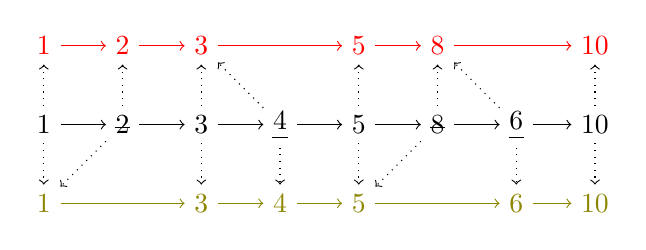
\begin{tikzpicture}
    \node (o1) {1};
    \node[right of=o1] (o2) {\st{2}};
    \node[right of=o2] (o3) {3};
    \node[right of=o3] (o4) {\ul{4}};
    \node[right of=o4] (o5) {5};
    \node[right of=o5] (o8) {\st{8}};
    \node[right of=o8] (o6) {\ul{6}};
    \node[right of=o6] (o10) {10};
    \draw[->] (o1) -- (o2);
    \draw[->] (o2) -- (o3);
    \draw[->] (o3) -- (o4);
    \draw[->] (o4) -- (o5);
    \draw[->] (o5) -- (o8);
    \draw[->] (o8) -- (o6);
    \draw[->] (o6) -- (o10);

    \node[red, above of=o1] (d1) {1};
    \node[red, above of=o2] (d2) {2};
    \node[red, above of=o3] (d3) {3};
    \node[red, above of=o5] (d5) {5};
    \node[red, above of=o8] (d8) {8};
    \node[red, above of=o10] (d10) {10};
    \draw[red, ->] (d1) -- (d2);
    \draw[red, ->] (d2) -- (d3);
    \draw[red, ->] (d3) -- (d5);
    \draw[red, ->] (d5) -- (d8);
    \draw[red, ->] (d8) -- (d10);
    \draw[dotted, ->] (o1) -- (d1);
    \draw[dotted, ->] (o2) -- (d2);
    \draw[dotted, ->] (o3) -- (d3);
    \draw[dotted, ->] (o4) -- (d3);
    \draw[dotted, ->] (o5) -- (d5);
    \draw[dotted, ->] (o8) -- (d8);
    \draw[dotted, ->] (o6) -- (d8);
    \draw[dotted, ->] (o10) -- (d10);

    \node[olive, below of=o1] (i1) {1};
    \node[olive, below of=o3] (i3) {3};
    \node[olive, below of=o4] (i4) {4};
    \node[olive, below of=o5] (i5) {5};
    \node[olive, below of=o6] (i6) {6};
    \node[olive, below of=o10] (i10) {10};
    \draw[olive, ->] (i1) -- (i3);
    \draw[olive, ->] (i3) -- (i4);
    \draw[olive, ->] (i4) -- (i5);
    \draw[olive, ->] (i5) -- (i6);
    \draw[olive, ->] (i6) -- (i10);
    \draw[dotted, ->] (o1) -- (i1);
    \draw[dotted, ->] (o2) -- (i1);
    \draw[dotted, ->] (o3) -- (i3);
    \draw[dotted, ->] (o4) -- (i4);
    \draw[dotted, ->] (o5) -- (i5);
    \draw[dotted, ->] (o8) -- (i5);
    \draw[dotted, ->] (o6) -- (i6);
    \draw[dotted, ->] (o10) -- (i10);
\end{tikzpicture}
\end{minipage}
\caption{Execution synchronization of a source and a destination program extracted from a difference tree without colors. For simplification, we show only one state for each line of code.}
\label{fig:oracle_sync_from_diff}
\end{figure}

Formally, the correlation oracle is defined as a program with a states that can be projected on either of the correlated programs. Moreover, it carries information about the co-execution of both programs.

Here we keep states as tuples $\langle\kappa, v, S\rangle$ but all the individual components are slightly more complex: $\kappa$ is the continuation but its elements can be either deleted (\st{$instr$}$^c$), inserted (\ul{$instr$}$^c$), or preserved ($instr$), depending on whether they occur on the original only, the merged candidate only or both. Deleted and inserted instructions carry a color with them. For each value $v$ or element of the store $S(x)$, they are replaced by a pair of values associated with a color $(v_{del}, v_{ins}, c)$.

The projection of a state to its equivalent in the original program $\pi_{del}$ removes all the inserted instructions in the continuation, and takes first elements of pairs of values, always ignoring colors. Same for the projection on the merge candidate $\pi_{ins}$, but removing deleted instructions, and taking second element inside pair of values.

For $S$ a store, we denote $S_{del} = \pi_{del} \circ S$, $S_{ins} = \pi_{ins} \circ S$ and $S_{c}$ the projection on the color of the value of $S$.

To describe how interleaving is done, we can also give operational semantic reductions. All the rules from the underlying language can be reused for instructions that simply expand inside the continuation. In this case we preserve the deleted/inserted/preserved status and the color on the expansion. For the rest, we have the following rules:
\begin{align*}
\langle \kappa, (v_d, v_i, \bot), S\rangle &\not\rightarrow\\
\langle x = \square \cdot \kappa, (v_d, v_i, c), S\rangle &\rightarrow \langle \kappa, (), S[x \leftarrow (v_d, v_i, c)]\rangle\\
\langle \text{\st{$x = \square$}}^k \cdot \kappa, (v_d, v_i, c), S\rangle &\rightarrow \langle \kappa, (), S[x \leftarrow (v_d, S_{ins}(x), S_c(x) \cap k)]\rangle\\
\langle \text{\ul{$x = \square$}}^k \cdot \kappa, (v_d, v_i, c), S\rangle &\rightarrow \langle \kappa, (), S[x \leftarrow (S_{del}(x), v_i, c \cap k)]\rangle\\
\langle x \cdot \kappa, (v_d, v_i, c), S\rangle &\rightarrow \langle \kappa, S(x), S\rangle\\
\langle \text{\st{$x$}}^k \cdot \kappa, (v_d, v_i, c), S\rangle &\rightarrow \langle \kappa, (S_{del}(x), v_i, c \cap k), S\rangle\\
\langle \text{\ul{$x$}}^k \cdot \kappa, (v_d, v_i, c), S\rangle &\rightarrow \langle \kappa, (v_d, S_{ins}(x), S_c(x) \cap k), S\rangle\\
\langle literal \cdot \kappa, (v_d, v_i, c), S\rangle &\rightarrow \langle \kappa, (literal, literal, \top), S\rangle\\
\langle \text{\st{$literal$}}^k \cdot \kappa, (v_d, v_i, c), S\rangle &\rightarrow \langle \kappa, (literal, v_i, c \cap k), S\rangle\\
\langle \text{\ul{$literal$}}^k \cdot \kappa, (v_d, v_i, c), S\rangle &\rightarrow \langle \kappa, (v_d, literal, k), S\rangle\\
\langle \star \square \cdot \kappa, (v_d, v_i, c), S\rangle &\rightarrow \langle \kappa, (\star v_d, \star v_i, c), S\rangle\\
\langle (v_d^1, v_i^1, c^1) \diamond \square \cdot \kappa, (v_d^2, v_i^2, c^2), S\rangle &\rightarrow \langle \kappa, (v_d^1 \diamond v_d^2, v_i^1 \diamond v_i^2, c^1 \cap c^2), S\rangle\\
\langle f(\overrightarrow{(v_d^a, v_i^a, c^a)}) \cdot \kappa, (v_d, v_i, c), S\rangle &\rightarrow \langle \mathbb{G}(f) \cdot \mathbf{eof} \cdot \kappa, (), \{\overrightarrow{a \leftarrow (v_d^a, v_i^a, c^a)}\} :: S\rangle\\
% \langle C(\overrightarrow{(v_d^a, v_i^a, c^a)}) \cdot \kappa, (v_d, v_i)^c, S\rangle &\rightarrow \langle \kappa, C(\overrightarrow{v_a}), S\rangle\\
\langle \mathbf{if}\ \square\ b_{true}\ \mathbf{else}\ b_{false} \cdot  \kappa, (\mathbf{true}, \mathbf{true}, \top), S\rangle &\rightarrow \langle b_{true} \cdot \kappa, (), S\rangle\\
\langle \mathbf{if}\ \square\ b_{true}\ \mathbf{else}\ b_{false} \cdot  \kappa, (\mathbf{false}, \mathbf{false}, \top), S\rangle &\rightarrow \langle b_{false} \cdot \kappa, (), S\rangle\\
\langle \mathbf{if}\ \square\ b_{true}\ \mathbf{else}\ b_{false} \cdot  \kappa, (v_d, v_i, c), S\rangle &\rightarrow \langle \text{\st{$\mathbf{if}\ \square\ b_{true}\ \mathbf{else}\ b_{false}$}}^c \cdot \text{\ul{$\mathbf{if}\ \square\ b_{true}\ \mathbf{else}\ b_{false}$}}^c \cdot \kappa, (v_d, v_i, c), S\rangle\\
\langle \text{\st{$\mathbf{if}\ \square\ b_{true}\ \mathbf{else}\ b_{false}$}}^k \cdot  \kappa, (\mathbf{true}, v_i, c), S\rangle &\rightarrow \langle \text{\st{$b_{true}$}}^k \cdot \kappa, ((), v_i, c), S\rangle \qquad \text{(also works with \textbf{false})}\\
\langle \text{\ul{$\mathbf{if}\ \square\ b_{true}\ \mathbf{else}\ b_{false}$}}^k \cdot \kappa, (v_d, \mathbf{true}, c), S\rangle &\rightarrow \text{\ul{$b_{true}$}}^{k \cap c} \cdot \kappa, (v_d, (), c), S\rangle \qquad \text{(also works with \textbf{false})}\\
% \langle \mathbf{match}\ \square\ \{ \overrightarrow{C(\overrightarrow{x_C,}) \Rightarrow e_C,} \} \cdot \kappa, D(\overrightarrow{v_D}), S\rangle &\rightarrow \langle e_D \cdot \kappa, (), S[\overrightarrow{x_D \leftarrow v_D}]\rangle\\
\langle \text{\st{\textbf{continue}}}^k \cdot \overrightarrow{\kappa_{\neg while}} \cdot \textbf{while}\ e_{cond}\ b \cdot \kappa, (v_d, v_i, c), S\rangle &\rightarrow \langle \overrightarrow{\text{\ul{$\kappa_{\neg while}$}}}^k \cdot \textbf{while}\ e_{cond}\ b \cdot \kappa, ((), v_i, c), S\rangle\\
\langle \text{\ul{\textbf{continue}}}^k \cdot \overrightarrow{\kappa_{\neg while}} \cdot \textbf{while}\ e_{cond}\ b \cdot \kappa, (v_d, v_i, c), S\rangle &\rightarrow \langle \overrightarrow{\text{\st{$\kappa_{\neg while}$}}}^k \cdot \textbf{while}\ e_{cond}\ b \cdot \kappa, (v_d, (), c), S\rangle\\
\langle \text{\st{\textbf{break}}}^k \cdot \overrightarrow{\kappa_{\neg while}} \cdot \textbf{while}\ e_{cond}\ b \cdot \kappa, (v_d, v_i, c), S\rangle &\rightarrow \langle \overrightarrow{\text{\ul{$\kappa_{\neg while}$}}}^k \cdot \text{\ul{$\textbf{while}\ e_{cond}\ b$}}^k \cdot \kappa, ((), v_i, c), S\rangle\\
\langle \text{\ul{\textbf{break}}}^k \cdot \overrightarrow{\kappa_{\neg while}} \cdot \textbf{while}\ e_{cond}\ b \cdot \kappa, (v_d, v_i, c), S\rangle &\rightarrow \langle \overrightarrow{\text{\st{$\kappa_{\neg while}$}}}^k \cdot \text{\st{$\textbf{while}\ e_{cond}\ b$}}^k \cdot \kappa, (v_d, (), c), S\rangle\\
\langle \text{\st{$\mathbf{return}\ \square$}}^k \cdot \overrightarrow{\kappa_{\neg eof}} \cdot \textbf{eof} \cdot \kappa, (v_d, v_i, c), S\rangle &\rightarrow \langle \overrightarrow{\text{\ul{$\kappa_{\neg eof}$}}}^k \cdot \textbf{eof} \cdot \kappa, (v_d, v_i, c), S\rangle\\
\langle \text{\ul{$\mathbf{return}\ \square$}}^k \cdot \overrightarrow{\kappa_{\neg eof}} \cdot \textbf{eof} \cdot \kappa, (v_d, v_i, c), S\rangle &\rightarrow \langle \overrightarrow{\text{\st{$\kappa_{\neg eof}$}}}^k \cdot \textbf{eof} \cdot \kappa, (v_d, v_i, c), S\rangle\\
\end{align*}

\todo{Add match and enum constructors to these rules}

If an instruction in the continuation should be both inserted and deleted according to the rules, it is simply discarded. If it should be deleted or inserted twice with different colors, we take the intersection of these colors.

\subsection{A key principle: mandatory disambiguation}
\paragraph{A generic definition of a valid merge} A merge is valid if for any state of the program, there is a single unambiguous trace after applying all the modifications of the concurrent commits. There should be no automatic choice in favor of any of the commits. This means that if two commits touched the same state of the program or the same expression at the same time, the merge will be considered not valid. We call a point in a trace where the semantic is ambiguous a collision.
Note that I consider that this includes a case where commit $A$ modifies a variable $x$ and then commit $B$ changes the value of $y$ to the new value of $x$.

\noindent
\begin{minipage}{.32\textwidth}
\begin{lstlisting}
// Commit A
let x = 2;
let y = 3;
\end{lstlisting}
\end{minipage}\hfill
\begin{minipage}{.32\textwidth}
\begin{lstlisting}
// Original
let x = 1;
let y = 3;
\end{lstlisting}
\end{minipage}\hfill
\begin{minipage}{.32\textwidth}
\begin{lstlisting}
// Commit B
let x = 1;
let y = x; // !!!
\end{lstlisting}
\end{minipage}
\vspace{-.4cm}
\begin{lstlisting}[label=lst:change_introducing_modified, caption={Colliding changes by using a variable modified by someone else}]
\end{lstlisting}

\paragraph{Origin graphs for functional programs} To keep track of potential collisions we can create a graph of origins that is updated between each program state. In a program where variables are never mutable, this graph has a node for each variable plus one node for each modification (labeled by the commit). Two nodes are linked by an edge if the value of a variable comes from the value of another variable or comes directly from a modification.

If at a given point of a program, a node of the origin graph is transitively linked to modifications of different concurrent commits, then there is a collision on the variable definition.

\begin{figure}[ht]
\centering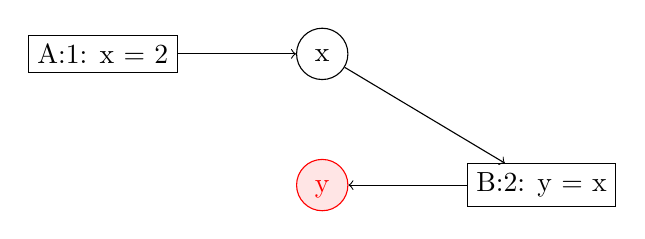
\begin{tikzpicture}
  \node[varnode] (x) {x};
  \node[varnode, below=1cm of x, conflict] (y) {y};

  \node[modnode, left=1.5cm of x] (x_A) {A:1: x = 2};
  \draw[->] (x_A) -- (x);

  \node[modnode, right=1.5cm of y] (y_B) {B:2: y = x};
  \draw[->] (x) -- (y_B);
  \draw[->] (y_B) -- (y);
\end{tikzpicture}
\caption{Illustration of the origin graph of the program showed in listing \ref{lst:change_introducing_modified}. There is a collision for $y$ because it is both linked to a modification in $A$ and a modification in $B$.}
\label{fig:change_introducing_modified}
\end{figure}

\begin{figure}[ht]
\begin{minipage}{.5\textwidth}
\begin{lstlisting}
let a = 0; // Modified by A
let b = 1; // Modified by B
let c = a + b; // Collision
\end{lstlisting}
\end{minipage}\hfill
\begin{minipage}{.45\textwidth}
\centering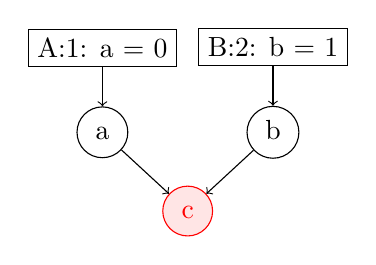
\begin{tikzpicture}
  \node[varnode] (a) {a};
  \node[varnode, right=1.5cm of a] (b) {b};
  \node[varnode, conflict] (c) at ($(a)!0.5!(b)+(0,-1)$) {c};

  \node[modnode, above=0.5cm of a] (A_a) {A:1: a = 0};
  \node[modnode, above=0.5cm of b] (B_b) {B:2: b = 1};

  \draw[->] (A_a) -- (a);
  \draw[->] (B_b) -- (b);
  \draw[->] (a) -- (c);
  \draw[->] (b) -- (c);
\end{tikzpicture}
\end{minipage}
\caption{Collision created after modification of two independent variables}
\end{figure}
\FloatBarrier

\paragraph{Origin graph and control flow} If the value of a variable is used for defining control flow, all the variables inside the branches will gain a dependency on it.

However incompatible branches can be treated independently and do not generate conflicts by themselves.

\begin{figure}[ht]
\begin{minipage}{.5\textwidth}
\begin{lstlisting}
let b = 2; // Modified by B
let x =
    if (c) {
        1 // Modified by A
    } else {
        b // Touched by B
    };
let y = x - 1; // OK
let z = y + b; // Conflict
\end{lstlisting}
\end{minipage}\hfill
\begin{minipage}{.45\textwidth}
\centering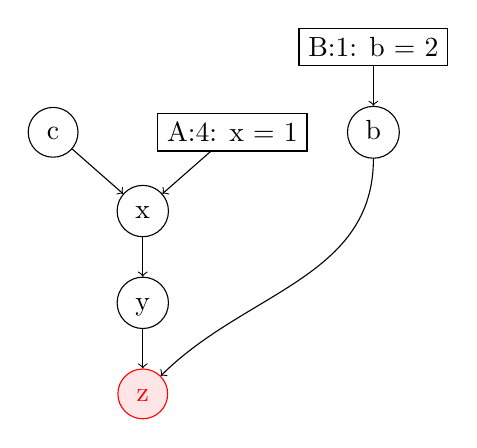
\begin{tikzpicture}
  \node[varnode] (b) {b};
  \node[modnode, above=0.5cm of b] (B_b) {B:1: b = 2};
  \node[modnode, left=0.5cm of b] (A_x) {A:4: x = 1};
  \node[varnode, left=1cm of A_x] (c) {c};
  \node[varnode] (x) at ($(c)!0.5!(A_x)+(0,-1)$) {x};
  \node[varnode, below=0.5cm of x] (y) {y};
  \node[varnode, below=0.5cm of y, conflict] (z) {z};


  \draw[->] (B_b) -- (b);
  \draw[->] (c) -- (x);
  \draw[->] (A_x) -- (x);
  \draw[->] (x) -- (y);
  \draw[->] (y) -- (z);
  \draw[->] (b) to[out=-90, in=45] (z);
\end{tikzpicture}
\end{minipage}
\caption{Origin graph at the end of a program after taking the then branch, showing that there is no collision on $x$ but still one on $z$.}
\label{fig:origin_graph_branches}
\end{figure}

This might become a problem if care is not taken in origin graph checks, because each branch combination might need to be examined.

\paragraph{Solving collisions by overriding}
In order to be able to solve collisions, I extend the definition of a merge with a set of modification overrides in addition to the set of concurrent commits.
A modification in the override set, take precedence over any modification in any of the merged commits. Moreover we can consider that these overrides are done knowing what is inside all the concurrent commits.

In the origin graph, a variable that takes a value defined in by an override modification will loose all incoming arrows as its value is now disambiguated for the current state, taking all further implications into account.

Having a single overridden ancestor can be not enough for marking a conflict as solved though.

\begin{figure}[ht]
\begin{minipage}{.5\textwidth}
\begin{lstlisting}
let a = 0; // modified by A
let b = 1; // modified by B
let o = a + b; // overriden
let c = a + o;
let d = c + b; // Collision!
\end{lstlisting}
\end{minipage}\hfill
\begin{minipage}{.45\textwidth}
\centering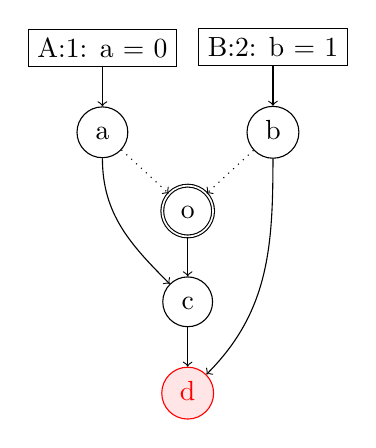
\begin{tikzpicture}
  \node[varnode] (a) {a};
  \node[varnode, right=1.5cm of a] (b) {b};
  \node[varnode, double] (o) at ($(a)!0.5!(b)+(0,-1)$) {o};
  \node[varnode, below=0.5cm of o] (c) {c};
  \node[varnode, below=0.5cm of c, conflict] (d) {d};

  \node[modnode, above=0.5cm of a] (A_a) {A:1: a = 0};
  \node[modnode, above=0.5cm of b] (B_b) {B:2: b = 1};

  \draw[->] (A_a) -- (a);
  \draw[->] (B_b) -- (b);
  \draw[->, dotted] (a) -- (o);
  \draw[->, dotted] (b) -- (o);
  \draw[->] (o) -- (c);
  \draw[->] (c) -- (d);
  \draw[->] (a) to[out=-90,in=135] (c);
  \draw[->] (b) to[out=-90,in=45] (d);
\end{tikzpicture}
\end{minipage}
\caption{Origin graph for a merge with an overriding that solves one conflict line 3 but is insufficient to also solve the conflict line 5. Deleted edges are dotted, variables overridden have a double border.}
\end{figure}

A override can arbitrarily alter a modification, or even touch something that was not modified to restore the intent of both modifications. In the example above, $o$ might have been untouched neither by $A$ or by $B$ or be touch by one of the commits or by both, it doesn't matter. That's why an override is also a way to state the behavior of the program when the changes are on the same state.

Usually there can be several way to solve the same conflict, but some are more ``powerful'' than others. A variable assigned to an overridden expression should be considered as a variable with a restored semantic with respect to all the modifications.

\begin{figure}[ht]
\begin{minipage}{.5\textwidth}
\begin{lstlisting}
let a = 0; // modified by A
let b = 1; // overriden
let o = a + b;
let c = a + o;
let d = c + b;
\end{lstlisting}
\end{minipage}\hfill
\begin{minipage}{.45\textwidth}
\centering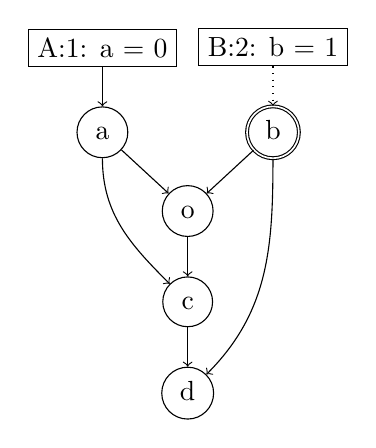
\begin{tikzpicture}
  \node[varnode] (a) {a};
  \node[varnode, right=1.5cm of a, double] (b) {b};
  \node[varnode] (o) at ($(a)!0.5!(b)+(0,-1)$) {o};
  \node[varnode, below=0.5cm of o] (c) {c};
  \node[varnode, below=0.5cm of c] (d) {d};

  \node[modnode, above=0.5cm of a] (A_a) {A:1: a = 0};
  \node[modnode, above=0.5cm of b] (B_b) {B:2: b = 1};

  \draw[->] (A_a) -- (a);
  \draw[->, dotted] (B_b) -- (b);
  \draw[->] (a) -- (o);
  \draw[->] (b) -- (o);
  \draw[->] (o) -- (c);
  \draw[->] (c) -- (d);
  \draw[->] (a) to[out=-90,in=135] (c);
  \draw[->] (b) to[out=-90,in=45] (d);
\end{tikzpicture}
\end{minipage}
\caption{Origin graph for the same example as before except that now line 2 is
overridden marking that $b$ has a preserved semantic. Therefore, line 5 is not showing a conflict anymore.}
\end{figure}

\subsection{From trace to program point origin graphs}
\paragraph{Graph coloring to check conflicts} For being able to quickly check that an assignment does not introduce a conflict, we can simply keep a coloring of the graph, that links each variable to the single unambiguous commit that modifies its semantic.
Therefore a well-formed graph without conflicts only have incoming edges from nodes without coloring or with the same color as itself.
Overridden variables will never be colored as they are considered to never collide with any of the concurrent commits.

\begin{figure}[ht]
\begin{minipage}{.5\textwidth}
\begin{lstlisting}
let b = 2; // Modified by B
let x =
    if (c) {
        1 // Modified by A
    } else {
        b // Touched by B
    };
let y = x - 1; // OK
let z = y + b; // Conflict
\end{lstlisting}
\end{minipage}\hfill
\begin{minipage}{.45\textwidth}
\centering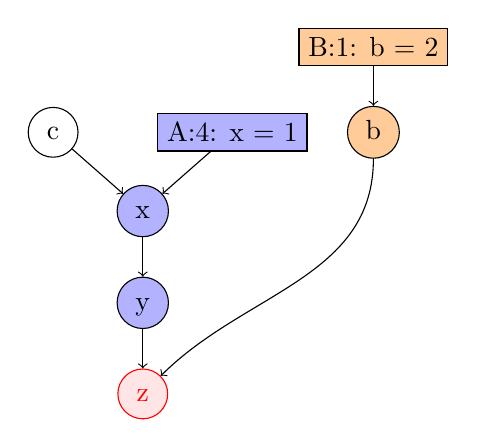
\begin{tikzpicture}
  \node[varnode, colorB] (b) {b};
  \node[modnode, above=0.5cm of b, colorB] (B_b) {B:1: b = 2};
  \node[modnode, left=0.5cm of b, colorA] (A_x) {A:4: x = 1};
  \node[varnode, left=1cm of A_x] (c) {c};
  \node[varnode, colorA] (x) at ($(c)!0.5!(A_x)+(0,-1)$) {x};
  \node[varnode, below=0.5cm of x, colorA] (y) {y};
  \node[varnode, below=0.5cm of y, conflict] (z) {z};


  \draw[->] (B_b) -- (b);
  \draw[->] (c) -- (x);
  \draw[->] (A_x) -- (x);
  \draw[->] (x) -- (y);
  \draw[->] (y) -- (z);
  \draw[->] (b) to[out=-90, in=45] (z);
\end{tikzpicture}
\end{minipage}
\caption{Same origin graph as figure \ref{fig:origin_graph_branches} with coloring}
\label{fig:origin_graph_branches_color}
\end{figure}

\paragraph{Program point origin graph} Also, to ease verification we need to switch from origins graph specified for a given trace to origin graphs specified at a given program point. In absence of control flow expressions, we have no problem for defining it as there is only one trace going from the beginning of the program to its end. However we need to deal with conditions and recursive calls (analogous to loops but in a functional setup) and arbitrary nesting of these two.

A good origin graph at a given program point must be projectable on any trace leading to the program point, and show conflict if at least one of the trace has a conflict.

\paragraph{Conditionals} Join after conditionals seems doable by creating a new color at the join point for each pair of distinct colors in the different branches. New colors should not be created if a variable is not colored in one branch or if it has the same color in both. In these case, it should retain its unambiguous color.

\begin{figure}[!ht]
\centering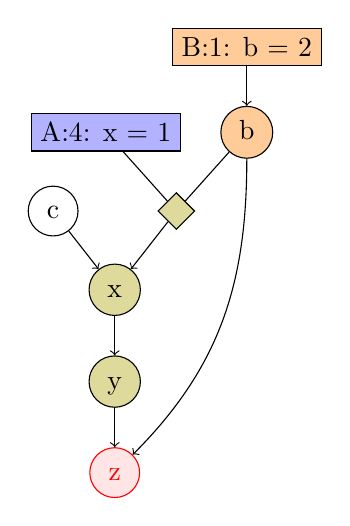
\begin{tikzpicture}
  \node[varnode, colorB] (b) {b};
  \node[modnode, above=0.5cm of b, colorB] (B_b) {B:1: b = 2};
  \node[modnode, left=0.5cm of b, colorA] (A_x) {A:4: x = 1};
  \node[condnode, colorC] (if) at ($(A_x)!0.5!(b)+(0,-1)$) {};
  \node[varnode, left=1cm of if] (c) {c};
  \node[varnode, colorC] (x) at ($(c)!0.5!(if)+(0,-1)$) {x};
  \node[varnode, below=0.5cm of x, colorC] (y) {y};
  \node[varnode, below=0.5cm of y, conflict] (z) {z};

  \draw[->] (B_b) -- (b);
  \draw[->] (c) -- (x);
  \draw (A_x) -- (if);
  \draw (b) -- (if);
  \draw[->] (if) -- (x);
  \draw[->] (x) -- (y);
  \draw[->] (y) -- (z);
  \draw[->] (b) to[out=-90, in=45] (z);
\end{tikzpicture}
\caption{Origin graph for program figure \ref{fig:origin_graph_branches_color} representing all paths going to line 9 at once. Diamonds represent joins after conditional blocks.}
\end{figure}

\begin{figure}[!ht]
\begin{minipage}{.35\textwidth}
\begin{lstlisting}
let x;
if (c) {
    x = 1; // A
} else {
    x = 2; // B
}
let y = x - 1;
let z = x + y;
let u;
if (d) {
    u = 3; // A
} else {
    u = 4; // B
}
let v = z + u; // !
\end{lstlisting}
\end{minipage}\hfill
\begin{minipage}{.6\textwidth}
\centering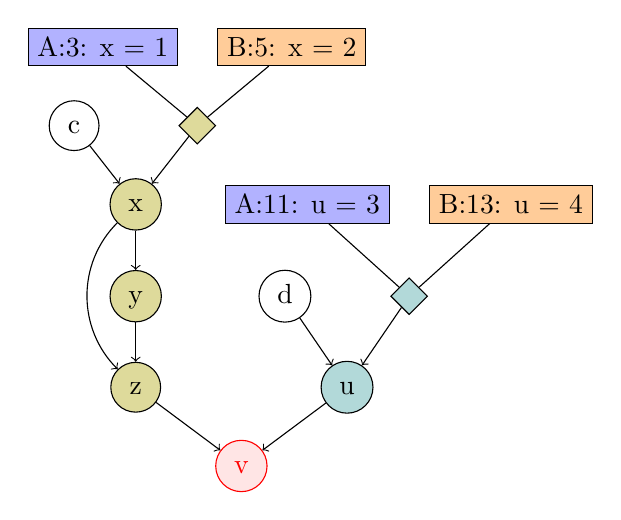
\begin{tikzpicture}
  \node[modnode, colorA] (A_x) {A:3: x = 1};
  \node[modnode, right=0.5cm of A_x, colorB] (B_x) {B:5: x = 2};
  \node[condnode, colorC] (if) at ($(A_x)!0.5!(B_x)+(0,-1)$) {};
  \node[varnode, left=1cm of if] (c) {c};
  \node[varnode, colorC] (x) at ($(c)!0.5!(if)+(0,-1)$) {x};
  \node[varnode, below=0.5cm of x, colorC] (y) {y};
  \node[varnode, below=0.5cm of y, colorC] (z) {z};

  \draw[->] (c) -- (x);
  \draw (A_x) -- (if);
  \draw (B_x) -- (if);
  \draw[->] (if) -- (x);
  \draw[->] (x) -- (y);
  \draw[->] (y) -- (z);
  \draw[->] (x) to[out=-135, in=135] (z);

  \node[modnode, right=0.8cm of x, colorA] (A_u) {A:11: u = 3};
  \node[modnode, right=0.5cm of A_u, colorB] (B_u) {B:13: u = 4};
  \node[condnode, colorD] (ifu) at ({$(A_u)!0.5!(B_u)$} |- y) {};
  \node[varnode, left=1cm of ifu] (d) {d};
  \node[varnode, colorD] (u) at ({$(d)!0.5!(ifu)$} |- z)  {u};
  \node[varnode, conflict] (v) at ($(z)!0.5!(u)+(0,-1)$) {v};

  \draw (A_u) -- (ifu);
  \draw (B_u) -- (ifu);
  \draw[->] (ifu) -- (u);
  \draw[->] (d) -- (u);
  \draw[->] (u) -- (v);
  \draw[->] (z) -- (v);
\end{tikzpicture}
\end{minipage}
\caption{Origin graph at the end of the program summarizing all the possible paths. There is a conflict on $v$ because for example if the green diamond is resolved in favor of $A$ and teal diamond is resolved in favor of $B$, we have an ambiguous value line 15.}
\label{fig:multiple_if}
\end{figure}

We can easily compute the projection on a trace that take a given path by choosing one of the two original colors as a replacement for each color created by merges (and remove the unmatching edges).

An explosion of the number of colors is impossible as the number of colors is bounded at a given point by the number of variables.

This strategy might incur a loss of precision by marking with different colors two distinct conditional expressions on the same condition but is a safe approximation. If necessary, we can refine this by remember the conditions involved to later check that indeed the conflicting case can happen, and print the conflicting path to the user.
\FloatBarrier

\paragraph{Handling recursive functions} In presence of functions we need to add a node for the return value of the function and also add nodes for each functions calls. For the moment, I consider that the result of a function call depends on all the arguments, and only that.

Recursive functions will create some kind of loop in the origin graph (that is representing the implicit looping control flow). Therefore in their presence, we have to be careful and do the coloring after the full construction of the origin graph.
\begin{figure}[!ht]
\begin{minipage}{.5\textwidth}
\begin{lstlisting}
fn f(l: List) -> i32 {
    match l {
        Nil => a,
        Cons(_, t) => b + f(t)
    }
}
\end{lstlisting}
\end{minipage}\hfill
\begin{minipage}{.45\textwidth}
\centering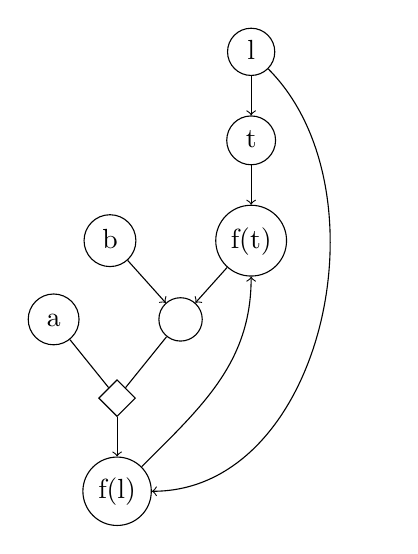
\begin{tikzpicture}
  \node[varnode] (l) {l};
  \node[varnode, below=0.5cm of l] (t) {t};
  \node[varnode, below=0.5cm of t] (ft) {f(t)};
  \node[varnode, left=1cm of ft] (b) {b};
  \node[varnode] (cons_tmp) at ($(ft)!0.5!(b)+(0,-1)$) {};
  \node[varnode, left=1cm of cons_tmp] (a) {a};
  \node[condnode] (switch) at ($(a)!0.5!(cons_tmp)+(0,-1)$) {};
  \node[varnode, below=0.5cm of switch] (res) {f(l)};

  \draw[->] (l) -- (t);
  \draw[->] (t) -- (ft);
  \draw[->] (ft) -- (cons_tmp);
  \draw[->] (b) -- (cons_tmp);
  \draw (a) -- (switch);
  \draw (cons_tmp) -- (switch);
  \draw[->] (switch) -- (res);
  \draw[->] (l) to[out=-45, in=0] (res);
  \draw[->] (res) to[out=45, in=-90] (ft);
\end{tikzpicture}
\end{minipage}
\caption{Origin graph of a recursive function.}
\label{fig:fun_rec}
\end{figure}


\paragraph{Higher order programs with closures} What happens if functions can be inside variables? Seems that simply considering that the function (and all its arguments) is a dependency of all its calls is enough.

We just need to be careful with captures. A conservative approach would consider that if a function captures a variable, then it gets a dependency on it. But this can create conflicts that do not exist, if captured variables are used in different branches. A more natural approach is to analyze the inside of the function in the definition environment and then keep the color of the result for the function itself at the end.

\begin{figure}[!ht]
\begin{minipage}{.5\textwidth}
\begin{lstlisting}
let a = 1; // Modified by A
let b = 2; // Modified by B
let f = |x, c| {
    if (c) {
        x + a
    } else {
        x + b
    }
};
let r = f(b, true);
\end{lstlisting}
\end{minipage}\hfill
\begin{minipage}{.45\textwidth}
\centering\begin{tikzpicture}
  \node[varnode, colorA] (a) {a};
  \node[varnode, right=1.5cm of a, colorB] (b) {b};
  \node[modnode, above=0.5cm of b, colorB] (B_b) {B:1: b = 2};
  \node[modnode, above=0.5cm of a, colorA] (A_a) {A:4: x = 1};
  \node[condnode, colorC] (if) at ($(A_x)!0.5!(b)+(0,-1)$) {};
  \node[varnode, below=0.5cm of if, colorC] (f) {f};
  \node[varnode, below=0.5cm of f, conflict] (r) {r};

  \draw[->] (A_a) -- (a);
  \draw[->] (B_b) -- (b);
  \draw (A_x) -- (if);
  \draw (b) -- (if);
  \draw[->] (if) -- (f);
  \draw[->] (f) -- (r);
  \draw[->] (b) to[out=-90, in=45] (r);
\end{tikzpicture}
\end{minipage}
\caption{Origin graph with a closure. The conflict could actually disappear if inlining of $f$ is applied.}
\label{fig:closure}
\end{figure}

\subsection{Oracles for structure preserving modifications}

\paragraph{Modification of expressions only} This idea works very well for commits that only consist of modifications of expressions and preserve the whole program structure (but maybe not the control flow).

If we number all the expressions used in a program, then a commit is a partial map from expression indices to new expressions (and same for the override list).

For conditional branches (\lstinline$if$ or \lstinline$match$), we can consider them both as expressions and as structure. Therefore we can either choose to replace them totally, or to only replace expressions of branches, condition and/or scrutinee.
Obviously, replacing the whole expression, is also a modification of all the branches.

\paragraph{Linking programs before and after commits} For any source program and set of structure preserving modification with matching indices, we can build a correlation oracle that links the program before and the program after the commit together.

The only problem here occurs with programs whose termination status is modified by the commit. To simplify our problem, we will consider first programs that do always terminate.

The correlation oracle can be constructed with as static environment the expression modifications and the origin graph at the end of the program, and as dynamic environment the state of the original program, and the store of the modified program.

The preserved invariant checks that only colored variables in the origin graph have a different value in the store of programs before and after the commit. It should also check the origin of values in the stack.

The interpretation function is executing programs in lockstep manner except that it has to perform a big step if there is a conditional with different conditions in different branches.

If a given program crashes because of a runtime exception, we have to continue executing the other one, relating all its following states to the crashing one.

\paragraph{A correlation oracle to check fusion} Suppose that we have already proven that there is an origin graph including all modifications of all the concurrent commits, with a given list of overrides.

TODO: finish that

\subsection{Checking imperative programs}

\paragraph{Origin graph and mutable variables} In presence of mutable variables we should track not variables but assignment expressions inside the origin graph, and separately keep a link from variables to their definition at the current program point.

\begin{figure}[ht]
\begin{minipage}{.5\textwidth}
\begin{lstlisting}
let a = 2;
let b = 5;
let mut c = a;
while (c < b) {
    c += 1;
}
\end{lstlisting}
\end{minipage}\hfill
\begin{minipage}{.45\textwidth}
\centering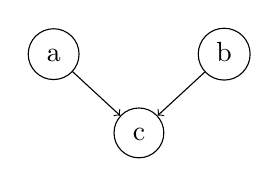
\begin{tikzpicture}
  \node[varnode] (a) {a};
  \node[varnode, right=1.5cm of a] (b) {b};
  \node[varnode] (c) at ($(a)!0.5!(b)+(0,-1)$) {c};

  \draw[->] (a) -- (c);
  \draw[->] (b) -- (c);
\end{tikzpicture}
\end{minipage}
\caption{Origin graph at the end of a program containing a while-loop. Note that $c$ keeps its dependency on $a$ as it used its previous value inside the loop.}
\end{figure}

\end{document}
